\documentclass[12pt]{report}

% ============================================================
% PAQUETES Y FORMATO SEGÚN GUÍA UTM
% ============================================================
\usepackage[utf8]{inputenc}
\usepackage[T1]{fontenc}
\usepackage[spanish]{babel}
\usepackage{helvet} % Fuente similar a Arial
\renewcommand{\familydefault}{\sfdefault}

% Márgenes: Sup, Inf, Der 2.5cm; Izq 3.5cm
\usepackage[left=3.5cm, right=2.5cm, top=2.5cm, bottom=2.5cm]{geometry}

% Interlineado 1.15
\usepackage{setspace}
\setstretch{1.15}

% Paquetes para gráficos, tablas y matemáticas
\usepackage{graphicx}
\usepackage{amsmath}
\usepackage{amssymb}
\usepackage{booktabs}
\usepackage{array}
\usepackage{multirow}
% Citas en formato autor-año (APA 7)
\usepackage[authoryear,round]{natbib}
\usepackage{hyperref}
\usepackage{tikz}
\usetikzlibrary{shapes.geometric, arrows, positioning}
\usepackage{float}
\usepackage{xcolor}
\usepackage{pdfpages}

% ------------------------------------------------------------
% CÓDIGO FUENTE CON RESALTADO DE SINTAXIS (Anexo A)
% ------------------------------------------------------------
\usepackage{listings}
\definecolor{codeblue}{rgb}{0.05,0.20,0.65}
\definecolor{codegreen}{rgb}{0.00,0.45,0.00}
\definecolor{codered}{rgb}{0.60,0.10,0.10}
\definecolor{codegray}{rgb}{0.45,0.45,0.45}
\definecolor{codebg}{rgb}{0.97,0.97,0.97}
\renewcommand{\lstlistingname}{Listado}
\lstdefinestyle{pythonstyle}{
    language=Python,
    % --- Fidelidad con el archivo original (indentación y espacios) ---
    columns=fullflexible,       % ancho natural de cada carácter: respeta la sangría
    keepspaces=true,            % conserva los espacios repetidos del código
    showstringspaces=false,     % no marca con símbolos los espacios en cadenas
    tabsize=4,                  % un tabulador equivale a cuatro espacios
    breaklines=true,            % parte las líneas que exceden el ancho
    breakatwhitespace=false,
    breakindent=2em,            % la continuación de una línea partida va sangrada
    % --- Presentación ---
    backgroundcolor=\color{codebg},
    basicstyle=\ttfamily\fontsize{9}{10.5}\selectfont,
    keywordstyle=\color{codeblue}\bfseries,
    commentstyle=\color{codegreen}\itshape,
    stringstyle=\color{codered},
    numberstyle=\scriptsize\color{codegray},
    numbers=left,
    numbersep=8pt,
    xleftmargin=17pt,
    framexleftmargin=17pt,
    frame=single,
    rulecolor=\color{codegray},
    captionpos=t,
    extendedchars=true,
    inputencoding=utf8,
}
\lstset{style=pythonstyle}

% Ruta de las imágenes (busca en la carpeta figs que está un nivel arriba)
\graphicspath{{../figs/}}

% Rotulación de tablas en español académico (APA: «Tabla», no «Cuadro»)
\addto\captionsspanish{%
  \renewcommand{\tablename}{Tabla}%
  \renewcommand{\listtablename}{Índice de tablas}%
  \renewcommand{\appendixname}{Anexo}%
}

% Formato de hipervínculos
\hypersetup{
    colorlinks=true,
    linkcolor=blue,
    urlcolor=blue,
    citecolor=blue
}

% ============================================================
% INICIO DEL DOCUMENTO
% ============================================================
\begin{document}

% ------------------------------------------------------------
% CARÁTULA (Sin numeración)
% ------------------------------------------------------------
\begin{titlepage}
    \centering
    \vspace*{2cm}
    {\LARGE\bfseries Universidad Tecnológica Metropolitana \par}
    \vspace{0.5cm}
    {\Large Maestría en Ciberseguridad \par}
    \vspace{2cm}
    {\Huge\bfseries Proyecto de Investigación Aplicada (PIA) \par}
    \vspace{1cm}
    % Título con máximo 15 palabras
    {\Large\bfseries Corrección de errores cuánticos y tasa de clave segura en el protocolo BB84 bajo canales ruidosos \par}
    \vspace{3cm}
    \begin{flushleft}
        \large
        \textbf{Estudiante:} Eliu Manuel Pat Ojeda \\
        \textbf{Matrícula:} 26011494 \\
        \textbf{Asesor:} Prof. Oscar Antonio Palma \\
        \textbf{Lugar y fecha:} Mérida, Yucatán. Noviembre de 2026.
    \end{flushleft}
    \vfill
\end{titlepage}

% ------------------------------------------------------------
% PRELIMINARES (Numeración romana)
% ------------------------------------------------------------
\pagenumbering{roman}

\chapter*{Resumen}
\addcontentsline{toc}{chapter}{Resumen}

Este proyecto de investigación aplicada aborda el compromiso (trade-off) entre la corrección de errores cuánticos (QEC) y la tasa de clave segura en el protocolo BB84 bajo un canal depolarizante. En el contexto de la amenaza del Q-Day, la Distribución de Claves Cuánticas (QKD) es una alternativa de seguridad. Sin embargo, su viabilidad depende de operar sobre canales ruidosos. Se implementó un simulador en Python y QuTiP para evaluar cómo el overhead de qubits de la QEC afecta la tasa efectiva de generación de clave. Los resultados demuestran que no existe un tamaño de código único óptimo, sino que depende del nivel de ruido del canal. Se identificó que para un ruido bajo no se requiere QEC, mientras que para ruidos moderados y altos, los códigos de 3 y 5 qubits maximizan la tasa efectiva, respectivamente, permitiendo decisiones de diseño informadas para infraestructuras de ciberseguridad cuántica.

\vspace{0.5cm}
\noindent \textbf{Palabras clave:} Ciberseguridad cuántica, QKD, Corrección de errores cuánticos, Protocolo BB84, Q-Day.

\tableofcontents
% \listoftables % Descomentar cuando tengas tablas
% \listoffigures % Descomentar cuando tengas figuras
\newpage

% ------------------------------------------------------------
% CUERPO DEL DOCUMENTO (Numeración arábiga)
% ------------------------------------------------------------
\pagenumbering{arabic}

\chapter{Problema y Fundamento}

\section{Introducción}

La seguridad de la infraestructura digital contemporánea descansa sobre un
conjunto reducido de supuestos matemáticos. Los esquemas de clave pública que
sostienen las comunicaciones cifradas, la firma electrónica, la banca en línea y
los sistemas de control industrial —RSA, Diffie-Hellman y la criptografía de
curva elíptica (ECC)— fundan su fortaleza en dos problemas que, para los tamaños
empleados en la práctica, ninguna computadora clásica puede resolver en un
tiempo razonable: descomponer un número en sus factores primos y hallar el
logaritmo discreto (es decir, averiguar a qué potencia hay que elevar un número
dado para obtener otro; la tarea equivale a abrir una caja fuerte probando
combinaciones, con un número de combinaciones tan enorme que la búsqueda
resulta inviable). \citet{shor1997} demostró que ambos problemas admiten solución
en tiempo polinómico —un tiempo que crece de forma moderada con el tamaño del
problema, en lugar de crecer de manera explosiva— sobre un computador cuántico
suficientemente grande y tolerante a fallos (capaz de operar correctamente
aunque sus componentes cometan errores). El horizonte temporal en que dicha
capacidad se encuentre disponible se designa, en la práctica profesional, como
\textit{Q-Day}: a partir de ese momento los algoritmos mencionados dejan de
ofrecer garantías de confidencialidad para los datos que protegen.

La amenaza, sin embargo, no pertenece únicamente al futuro. La estrategia
conocida como \textit{Harvest Now, Decrypt Later} (HNDL) consiste en interceptar
y archivar tráfico cifrado en el presente para descifrarlo cuando se disponga de
capacidad cuántica \citep{mosca2018}; equivale a guardar una carta cifrada con la
esperanza de encontrar algún día la manera de abrirla. Esta táctica convierte el
riesgo en un problema de seguridad actual, pues el criterio decisivo no es la
fecha del Q-Day, sino la relación entre el tiempo requerido para migrar la
infraestructura y el periodo durante el cual los datos deben permanecer secretos.
Cuando el segundo excede al primero, la información ya se encuentra comprometida
aunque su contenido aún no pueda leerse. Historiales clínicos, expedientes
gubernamentales, secretos industriales y registros financieros conservan valor
durante décadas, de modo que su intercepción presente constituye una pérdida
diferida pero efectiva. Por esa razón, el informe NIST IR 8547 \citep{nist2026ir}
recomienda iniciar la transición criptográfica antes de que exista una amenaza
operativa confirmada, y no cuando el Q-Day haya sido anunciado.

La respuesta institucional se ha articulado en torno a la criptografía
post-cuántica (PQC). En agosto de 2024, el National Institute of Standards and
Technology (NIST) publicó los primeros estándares federales de algoritmos
resistentes a ataques cuánticos: FIPS 203, que especifica el mecanismo de
encapsulamiento de claves ML-KEM \citep{nist2024a} —el procedimiento mediante el
cual dos partes acuerdan una clave secreta compartida sin haberla intercambiado
previamente—, y FIPS 204, que especifica el esquema de firma digital ML-DSA
\citep{nist2024b}. El informe NIST IR 8547 complementa esos estándares con un
plan de transición que contempla la retirada progresiva de RSA y ECC de los
sistemas federales \citep{nist2026ir}. La PQC constituye, no obstante, una
solución algorítmica: su seguridad vuelve a descansar en supuestos de
complejidad computacional que, aunque más robustos, no resultan indemnes a
futuros avances del cómputo cuántico ni a la criptoanálisis clásica.

Frente a ese enfoque, la distribución de claves cuánticas (QKD) propone un
fundamento distinto: la seguridad se deriva de las leyes de la mecánica cuántica
y no de la dificultad de un problema matemático. El protocolo BB84, formulado por
\citet{bennett1984}, permite a dos partes establecer una clave compartida
mediante la transmisión de estados cuánticos codificados en dos bases no
ortogonales (dos maneras incompatibles de medir un mismo qubit, algo así como
preguntar por el color o por la forma de un objeto: la respuesta a una de las
preguntas altera la respuesta a la otra). Su seguridad se apoya en el teorema de
no-clonación —no es posible copiar un estado cuántico desconocido sin alterar el
original, igual que no se puede fotocopiar un documento que se destruye al
fotocopiarlo— y en la perturbación inevitable de la medición, de modo que
cualquier intento de interceptación introduce errores detectables
\citep{gisin2002}. La seguridad incondicional del protocolo fue demostrada por
\citet{shor2000}, y revisiones posteriores han precisado sus condiciones de
seguridad práctica y las limitaciones de las implementaciones reales
\citep{scarani2009, xu2020, pirandola2020, lo2014}.

La viabilidad de la QKD depende, sin embargo, de la calidad del canal. En fibra
óptica, la atenuación, la decoherencia —la pérdida de las propiedades cuánticas
por interacción con el entorno, semejante a cómo una conversación se vuelve
ininteligible en una sala ruidosa—, el desalineamiento de los moduladores y las
cuentas oscuras de los detectores (detecciones falsas que el propio instrumento
registra aunque no haya llegado ningún qubit) introducen discrepancias entre los
bits preparados por Alice y los medidos por Bob \citep{xu2020}. Esas discrepancias
se cuantifican mediante la tasa de error de bit cuántico (QBER), una proporción
sencilla de interpretar: si de cada cien bits llegan alterados cuatro, el QBER
es del 4\,\%. Su valor condiciona la fracción de bits que puede convertirse en
clave secreta: superado un umbral cercano al 11\,\%, la tasa de clave segura se
anula \citep{shor2000}. La corrección de errores cuánticos (QEC) constituye el
mecanismo que permite operar por debajo de ese umbral, al distribuir la
información en varios qubits físicos y corregir los errores detectados
\citep{nielsen2010, terhal2015}. Su madurez tecnológica quedó demostrada con la
supresión del error lógico por debajo del umbral del código de superficie en un
procesador superconductor \citep{google2025}.

La corrección, no obstante, tiene un costo en recursos. Un código de repetición
de $n$ qubits emplea $n$ qubits físicos para transmitir un solo qubit lógico, de
modo que la tasa efectiva de clave queda penalizada por un factor $1/n$. Se
configura así un compromiso: incrementar $n$ reduce el QBER residual, pero
también reduce el número de bits de clave generados por qubit transmitido
\citep{fowler2012, jayachandran2025}. Como ambos efectos operan en direcciones
opuestas, la tasa efectiva no es monótona en $n$ —no crece indefinidamente al
aumentar el tamaño del código— y cabe esperar, para cada nivel de ruido, un
tamaño de código que la maximice. Identificar ese tamaño y cuantificar su
dependencia respecto del ruido constituye el problema central del presente
proyecto. La Sección~\ref{sec:tradeoff} desarrolla este compromiso con una imagen
intuitiva.

El propósito de esta investigación aplicada es analizar el impacto de la
corrección de errores cuánticos sobre la tasa de clave segura efectiva del
protocolo BB84 en un canal depolarizante, con el fin de determinar el tamaño de
código que maximiza dicha tasa en distintos regímenes de ruido. El estudio se
acota a un simulador desarrollado en Python con la biblioteca QuTiP
\citep{qutip2012}, a un modelo de ruido depolarizante y a códigos de repetición
con $n \in \{1, 3, 5, 7\}$. Los resultados se orientan a ofrecer criterios de
dimensionamiento verificables para el diseño de enlaces de QKD.

El documento se organiza en tres capítulos. El presente expone el problema, los
antecedentes y el marco teórico, la pregunta de investigación, los objetivos y
la justificación con su alcance y delimitaciones. El segundo describe el modelo
del sistema, la estrategia metodológica, la hipótesis de trabajo y la matriz de
congruencia. El tercero presenta los recursos, el cronograma, los resultados, la
discusión, las conclusiones y las limitaciones del proyecto.

El código fuente del simulador se incorpora en el Anexo~A, y el artículo
académico derivado de esta investigación, en el Anexo~B. Ambos anexos completan
la evidencia del proyecto y remiten, respectivamente, al repositorio de
evidencias y a la versión de comunicación científica de los resultados aquí
expuestos.

\section{Antecedentes y marco teórico}

Esta sección integra el estado del arte focalizado y los conceptos que sustentan
las decisiones metodológicas del proyecto. Se presentan, en primer término, los
fundamentos de la información cuántica y el protocolo BB84; en segundo término,
la corrección de errores cuánticos; finalmente, el compromiso entre corrección y
\textit{overhead} que da lugar a la pregunta de investigación. Los conceptos se
introducen en la medida en que se emplean en el desarrollo del modelo; no se
acumulan definiciones sin uso posterior.

\subsection{El qubit y el formalismo de la información cuántica}

La unidad de información de la computación clásica es el bit, que admite dos
valores mutuamente excluyentes. La unidad de la información cuántica es el
\textbf{qubit}, un sistema cuyo estado puede describirse como una combinación
lineal de dos estados base:
\begin{equation}
|\psi\rangle = \alpha|0\rangle + \beta|1\rangle,
\label{eq:qubit}
\end{equation}
con $\alpha, \beta \in \mathbb{C}$ y $|\alpha|^2 + |\beta|^2 = 1$
\citep{nielsen2010}. Los coeficientes $\alpha$ y $\beta$ son amplitudes de
probabilidad: números que, elevados al cuadrado, indican la probabilidad de
obtener $0$ o $1$ al medir el sistema en la base computacional.

Para un lector no especialista resulta útil una analogía habitual en la
divulgación: un bit es como un interruptor, que está encendido o apagado,
mientras que un qubit es como una \textbf{moneda girando en el aire}. Mientras
gira, la moneda no es cara ni cruz, sino una mezcla de ambas posibilidades; solo
al atraparla y mirarla se define un resultado. Conviene precisar, para no
distorsionar la física, que la moneda no contiene las dos respuestas a la vez: lo
que describe la superposición es la probabilidad de cada resultado y la relación
entre ambas, de modo que el resultado permanece indefinido hasta la medición. La
superposición, por tanto, no consiste en almacenar simultáneamente ambos valores
clásicos, sino en una descripción probabilística cuyo resultado se define
únicamente al medir.

Cuando el sistema interactúa con su entorno, el estado puro deja de ser una
descripción suficiente y se recurre a la \textbf{matriz de densidad} $\rho$, que
representa tanto estados puros como mezclas estadísticas:
\begin{equation}
\rho = \sum_i p_i |\psi_i\rangle\langle\psi_i|, \qquad \mathrm{Tr}(\rho) = 1,
\label{eq:densidad}
\end{equation}
y cuya entropía de von Neumann, $S(\rho) = -\mathrm{Tr}(\rho \log_2 \rho)$,
cuantifica la incertidumbre asociada al estado \citep{nielsen2010}. En términos
llanos, la matriz de densidad es una forma de describir el estado cuando no se
conoce con certeza —por ejemplo, «el qubit está en el estado $A$ con probabilidad
0{,}7 y en el estado $B$ con probabilidad $0{,}3$»— en lugar de una única
descripción exacta; la entropía de von Neumann mide, en esa descripción, cuánta
incertidumbre permanece. Dos propiedades adicionales resultan decisivas para la
criptografía cuántica. La primera es el \textbf{teorema de no-clonación}, que
prohíbe construir una copia idéntica de un estado cuántico desconocido. La
segunda es la \textbf{indistinguibilidad de estados no ortogonales}, que impide
discriminar con certeza entre dos estados cuyo producto interno no es nulo (dos
estados «parecidos» no pueden separarse con una sola medición, igual que dos
tonos de gris casi idénticos no se distinguen a simple vista). Ambas propiedades
sostienen la seguridad de los protocolos de QKD, pues cualquier estrategia de un
adversario que pretenda extraer información debe perturbar el estado transmitido.

\subsection{El protocolo BB84 y la tasa de clave segura}

El protocolo BB84, propuesto por \citet{bennett1984}, fue el primer esquema de
distribución de claves cuánticas y continúa siendo el más estudiado. Alice
codifica cada bit en uno de cuatro estados, seleccionando de manera aleatoria
una de dos bases mutuamente no ortogonales: la base $Z$, formada por
$\{|0\rangle, |1\rangle\}$, y la base $X$, formada por
$\{|+\rangle, |-\rangle\}$, con
$|\pm\rangle = (|0\rangle \pm |1\rangle)/\sqrt{2}$. Puede imaginarse cada base
como una «rejilla de lectura» distinta: un qubit preparado para una rejilla se
lee correctamente solo si se mide con esa misma rejilla, y al usar la otra el
resultado es parcialmente aleatorio. Bob mide cada qubit en una base elegida de
forma independiente y anuncia su elección; Alice conserva únicamente los bits en
los que ambas bases coinciden. El procedimiento comprende las etapas siguientes:

\begin{enumerate}
    \item \textbf{Preparación.} Alice genera un bit aleatorio $b$ y una base
    aleatoria $B \in \{Z, X\}$, y prepara el estado correspondiente.
    \item \textbf{Transmisión.} Los qubits atraviesan el canal cuántico, donde
    quedan expuestos al ruido y a una eventual interceptación.
    \item \textbf{Medición.} Bob mide cada qubit en una base $B'$ elegida al
    azar y registra el resultado $b'$.
    \item \textbf{Cribado.} Mediante un canal clásico autenticado, ambas partes
    comparan las bases y conservan solo los bits en los que coincidieron
    ($B = B'$), que forman la clave bruta; el resto se descarta porque su
    lectura es poco fiable.
    \item \textbf{Estimación del QBER.} Se revela una muestra de la clave bruta
    para estimar la tasa de error de bit cuántico.
    \item \textbf{Post-procesamiento.} Se aplican corrección de errores
    (reconciliación) y amplificación de privacidad —un procedimiento que
    condensa la clave en menos bits para eliminar cualquier información parcial
    que el adversario pudiera tener— para obtener la clave final.
\end{enumerate}

La elección entre dos bases no ortogonales es el núcleo de la seguridad: un
adversario que mida en la base incorrecta introduce errores que Alice y Bob
detectan durante la estimación del QBER \citep{gisin2002}. \citet{shor2000}
demostraron que la seguridad del protocolo puede reducirse a la de un código de
corrección de errores cuánticos y establecieron que, en el límite asintótico y
bajo el límite de información de Holevo (el máximo de información clásica
extraíble), la fracción de bits aprovechables como
clave secreta satisface
\begin{equation}
R = 1 - 2H_2(\mathrm{QBER}),
\qquad
H_2(x) = -x\log_2 x - (1-x)\log_2(1-x),
\label{eq:shor}
\end{equation}
donde $H_2$ es la entropía binaria de Shannon, es decir, la incertidumbre de una
variable con dos resultados posibles. El factor $2H_2(\mathrm{QBER})$
representa la información que debe sacrificarse para corregir errores y eliminar
el conocimiento del adversario. De esta expresión se sigue que la tasa es
positiva solo si $\mathrm{QBER} < 11$\,\% aproximadamente, umbral que fija el
límite operativo del protocolo. Formulaciones más generales de la cota de clave
secreta conducen a la misma dependencia funcional \citep{devetak2005}.

Para el modelo de ruido adoptado en este proyecto, el QBER admite una expresión
analítica. El \textbf{canal depolarizante} actúa sobre un qubit según
\begin{equation}
\mathcal{E}(\rho) = (1-p)\rho + \frac{p}{3}\left(X\rho X + Y\rho Y + Z\rho Z\right),
\label{eq:canal}
\end{equation}
donde $p \in [0,1]$ es la probabilidad de que ocurra un error de Pauli y cada
uno de los tres operadores $X$, $Y$ y $Z$ se aplica con probabilidad $p/3$
\citep{nielsen2010}. Conviene imaginar este canal como una línea telefónica que,
con probabilidad $p$, estropea la señal recibida de una de tres maneras
básicas: invierte el valor del bit ($X$), invierte su fase ($Z$) o produce ambas
alteraciones a la vez ($Y$); con probabilidad $1-p$ la señal llega intacta. En
BB84, cuando el estado se prepara en la base $Z$ un error de bit se produce si el
qubit sufre $X$ o $Y$, mientras que un error $Z$ altera únicamente la fase y deja
intacto el valor medido; en la base $X$ ocurre lo simétrico. En ambos casos la
probabilidad de discrepancia entre Alice y Bob es
\begin{equation}
\mathrm{QBER} = \frac{2}{3}p,
\label{eq:qber}
\end{equation}
relación que permite contrastar la simulación con la predicción teórica
\citep{gisin2002} y que se emplea en este trabajo como criterio de validación.

\subsection{Corrección de errores cuánticos}

La corrección de errores en el dominio cuántico no puede apoyarse en la
redundancia clásica ingenua, pues el teorema de no-clonación impide copiar un
estado arbitrario. La solución consiste en codificar un qubit lógico en un
subespacio de un sistema de mayor dimensión —un «rincón» reservado del espacio de
estados, donde se aloja la información válida—, de manera que los errores
localizados conduzcan al estado fuera de ese subespacio y puedan detectarse sin
medir la información codificada \citep{nielsen2010, roffe2019}. El formalismo de
los \textbf{códigos estabilizadores} unifica esta idea: el espacio de código se
define como un conjunto de estados que se mantienen intactos ante ciertas
mediciones (formalmente, el autoespacio de autovalor $+1$ de un subgrupo
abeliano del grupo de Pauli). Al preguntarle al sistema «¿está todo en orden?»,
tales mediciones responden siempre «sí» mientras no haya errores, y esa
respuesta colectiva define el espacio válido, sin revelar el valor lógico
almacenado. La medición de sus generadores proporciona el \textbf{síndrome}, un
conjunto de bits que funciona como el código de avería de un electrodoméstico:
indica qué falló y en qué posición, pero no dice para qué se estaba usando el
aparato \citep{gottesman1997}.

Sobre ese formalismo se construyeron los códigos CSS, que combinan códigos
clásicos para la protección frente a errores de bit y de fase —dos familias de
fallos que se corrigen por vías separadas— \citep{calderbank1996, steane1996}, y
los códigos de superficie, que ofrecen umbrales de error relativamente altos y un
\textit{overhead} que escala de forma favorable con la distancia del código (el
número mínimo de qubits que un error debe afectar para pasar inadvertido)
\citep{fowler2012, terhal2015}. La viabilidad experimental de esta familia quedó
demostrada por \citet{google2025}, quienes reportaron supresión del error lógico
por debajo del umbral en un procesador superconductor de 105 qubits.

El código empleado en este proyecto es el \textbf{código de repetición} de $n$
qubits, el más simple de la familia y el más adecuado para aislar el efecto del
\textit{overhead}. Su principio es la votación: si se envía el mismo valor tres,
cinco o siete veces, la mayoría conservará el valor correcto aunque alguno de los
envíos se altere. Codifica los estados lógicos como
\begin{equation}
|0\rangle_L = |00\cdots 0\rangle, \qquad |1\rangle_L = |11\cdots 1\rangle,
\label{eq:codigo}
\end{equation}
y su estabilizador está generado por los operadores $g_i = Z_iZ_{i+1}$, con
$i = 1, \ldots, n-1$. La medición de esos generadores produce un síndrome de
$n-1$ bits que identifica el qubit afectado por un error de bit, tras lo cual se
aplica la corrección correspondiente y se decodifica por votación mayoritaria
\citep{nielsen2010}. El código corrige hasta $t = \lfloor (n-1)/2 \rfloor$
errores de bit y, bajo el supuesto de errores independientes con probabilidad
$q$ por qubit físico, su probabilidad de fallo lógico es
\begin{equation}
P_{\text{fallo}}(n,q) = \sum_{k=\lceil n/2 \rceil}^{n} \binom{n}{k}
q^{k}(1-q)^{n-k}.
\label{eq:fallo}
\end{equation}
Esta expresión constituye el modelo analítico de referencia del código; su
contraste con los valores obtenidos por la implementación se presenta en el
Capítulo III. Cabe precisar que el código de repetición protege únicamente
frente a errores de bit, por lo que su aplicación en BB84 exige considerar por
separado el efecto de los errores de fase.

\subsection{El compromiso entre corrección y \textit{overhead}}
\label{sec:tradeoff}

La protección tiene un costo cuantificable en qubits. Si se define el factor de
eficiencia del código como $\eta(n) = 1/n$ —el recíproco del número de qubits
físicos necesarios por qubit lógico—, ese factor penaliza la tasa de clave.
Combinándolo con la cota de Shor-Preskill se obtiene la \textbf{tasa de clave
efectiva}:
\begin{equation}
R_{\text{efectiva}}(p,n)
= \frac{1}{n}\left[1 - 2H_2\left(\mathrm{QBER}_{\text{QEC}}(p,n)\right)\right].
\label{eq:efectiva}
\end{equation}

Este compromiso (\textit{trade-off}) admite una imagen intuitiva: la de
\textbf{contratar guardias de seguridad} para proteger un edificio. Si el barrio
es tranquilo —poco ruido en el canal—, basta con uno o dos guardias; sumar más no
aporta una protección apreciable y sí encarece la operación. Si la amenaza es
alta —mucho ruido—, un solo guardia resulta insuficiente y el edificio queda
expuesto, por lo que conviene contratar más. En la QEC, los «guardias» son los
qubits físicos adicionales que acompañan a cada qubit lógico: $n = 3$ significa
tres qubits físicos por cada valor lógico que se desea proteger. El objetivo no
es contratar al mayor número posible, sino el número suficiente para el nivel de
amenaza, porque cada guardia adicional consume recursos que dejan de destinarse
a transmitir información. Esta es exactamente la estructura de la ecuación
anterior: el corchete representa la protección efectiva —que mejora con $n$— y el
factor $1/n$ representa el costo de contratar esa protección.

La inspección de la expresión revela el compromiso que motiva la investigación:
al aumentar $n$, el término $\mathrm{QBER}_{\text{QEC}}$ decrece y la tasa bruta
se aproxima a la unidad, pero el factor $1/n$ reduce proporcionalmente el
rendimiento. Para un nivel de ruido bajo, la corrección aporta una mejora
marginal que no compensa el costo; para un nivel de ruido alto, la corrección
resulta imprescindible porque sin ella la tasa bruta se anula. Entre ambos
extremos debe existir un tamaño de código que maximice el producto.

La literatura reciente ha abordado distintos componentes de este problema, pero
no la determinación sistemática del óptimo. \citet{jha2024} propusieron integrar
el cifrado y la corrección de errores mediante códigos CSS, con el objetivo de
reducir el costo total al reunir ambas funciones en un mismo proceso.
\citet{zheng2024} desarrollaron una métrica de fidelidad de canal casi óptima
—una medida de qué tan parecido llega el estado emitido al estado recibido— que
permite evaluar el desempeño de un código sin resolver problemas de optimización
costosos. \citet{matsui2025} construyeron códigos asistidos por entrelazamiento
(un recurso de correlación entre partículas que carece de equivalente clásico) a
partir de códigos cuasi-cíclicos con duales complementarios, cuyas propiedades
resultan relevantes para mitigar la fuga de información a través de los
síndromes. En el plano experimental, el equipo de Google Quantum AI
\citep{google2025} demostró la corrección por debajo del umbral en hardware
superconductor, y \citet{jayachandran2025} validaron la aplicación de QEC en
BB84, reportando la reducción del QBER y el consiguiente incremento de la tasa de
clave. La Tabla~\ref{tab:antecedentes} sintetiza el alcance y las limitaciones de
esos trabajos respecto del problema aquí planteado.

\begin{table}[H]
\centering
\caption{Síntesis comparativa de los antecedentes directos.}
\label{tab:antecedentes}
\footnotesize
\begin{tabular}{@{}>{\raggedright\arraybackslash}p{2.8cm}>{\raggedright\arraybackslash}p{3.3cm}>{\raggedright\arraybackslash}p{4.1cm}>{\raggedright\arraybackslash}p{4.0cm}@{}}
\toprule
\textbf{Trabajo} & \textbf{Objeto de estudio} & \textbf{Método o aporte principal} & \textbf{Limitación respecto de este proyecto} \\
\midrule
Jha et al. (2024) & Integración de cifrado y corrección de errores en comunicación cuántica & Códigos CSS que cumplen ambas funciones en un mismo proceso & No analiza el tamaño de código óptimo ni la tasa efectiva frente al ruido en BB84 \\
\addlinespace
Zheng et al. (2024) & Evaluación del desempeño de códigos QEC & Métrica de fidelidad de canal casi óptima, computacionalmente eficiente & Evalúa fidelidad; no incorpora el \textit{overhead} de qubits ni la tasa de clave \\
\addlinespace
Matsui y Kaneko (2025) & Códigos QEC asistidos por entrelazamiento & Códigos cuasi-cíclicos con duales complementarios, con propiedades ante la fuga por síndromes & No se evalúa en BB84 ni se cuantifica el costo en qubits \\
\addlinespace
Acharya et al. (2025) & Corrección de errores en hardware superconductor (Google Quantum AI) & Código de superficie con supresión del error lógico bajo el umbral en 105 qubits & Orientado a computación; alto \textit{overhead} y sin análisis de la tasa de clave en QKD \\
\addlinespace
Jayachandran y Malathi (2025) & Aplicación de QEC al protocolo BB84 & Validación de la reducción del QBER y del incremento de la tasa de clave & No determina el tamaño de código óptimo ni el efecto sistemático del \textit{overhead} \\
\bottomrule
\end{tabular}
\end{table}

Del contraste anterior se desprende un vacío concreto: los trabajos revisados
acreditan que la QEC mejora la fiabilidad y que puede incrementar la tasa de
clave, pero ninguno establece, para el protocolo BB84, la frontera que relaciona
el nivel de ruido con el tamaño de código que maximiza la tasa efectiva. Esa
frontera es la que este proyecto se propone determinar.

\section{Problemática}

En los enlaces de QKD reales el QBER nunca es nulo. La atenuación de la fibra, la
decoherencia, el desalineamiento de los componentes ópticos y las cuentas oscuras
de los detectores producen tasas de error que, en condiciones experimentales,
suelen situarse entre el 1\,\% y el 10\,\% \citep{xu2020, scarani2009}. Esa
magnitud no constituye un detalle instrumental: de ella depende directamente la
fracción de bits que sobrevive al post-procesamiento. Sustituyendo la
Ecuación~\eqref{eq:qber} en la Ecuación~\eqref{eq:shor} se obtiene que, sin
corrección de errores, la tasa de clave se anula cuando $p \approx 0.165$. Las
corridas preliminares registradas para este proyecto
(\texttt{data/resultados\_finales.csv}) confirman ese comportamiento: en
$p = 0.16$ la tasa efectiva se reduce a $0.046$ y en $p = 0.18$ se anula,
aun cuando el canal todavía transmite estados con fidelidad apreciable. Un enlace
operado en ese régimen resulta inservible para generar clave, aunque el hardware
funcione conforme a especificación.

La corrección de errores cuánticos revierte esa situación, pero su efecto no es
gratuito. En las mismas corridas, para $p = 0.06$ el código de repetición con
$n = 3$ reduce el QBER de $0.040$ a $0.003$, es decir, más de un orden de
magnitud, y desplaza el umbral de seguridad más allá de $p = 0.30$, fuera del
rango estudiado. Sin embargo, la tasa efectiva en ese mismo punto desciende de
$0.514$ (sin QEC) a $0.314$ (con $n = 3$): la corrección mejora la calidad de
la clave y simultáneamente reduce la cantidad de clave obtenida por qubit
transmitido. El signo del balance depende del nivel de ruido. Mientras que en
$p = 0.02$ prescindir de la corrección multiplica por más de dos la tasa
efectiva, en $p = 0.18$ prescindir de ella conduce a una tasa nula. El barrido
preliminar sitúa el cruce entre ambas estrategias en torno a $p = 0.10$, donde
las tasas son prácticamente iguales ($0.265$ frente a $0.260$), y muestra que
a partir de $p = 0.20$ el óptimo se desplaza hacia $n = 5$ y, en $p \geq 0.28$,
hacia $n = 7$.

El problema que se aborda, por tanto, no consiste en decidir si conviene aplicar
corrección de errores, sino en determinar qué tamaño de código conviene aplicar
para cada nivel de ruido. En los términos de la analogía anterior, no se trata de
decidir si se contrata seguridad, sino cuántos guardias hacen falta en cada
barrio. La decisión es sensible: elegir $n = 3$ cuando el canal
presenta $p = 0.02$ desperdicia más de la mitad de la capacidad de generación
de clave, mientras que elegir $n = 1$ cuando $p = 0.18$ anula por completo la
generación. Ninguna de las dos elecciones puede justificarse sin un criterio
explícito que relacione el ruido observado con el costo en qubits.

La literatura revisada no proporciona ese criterio de forma sistemática. Los
trabajos que validan la QEC en BB84 reportan mejoras del QBER y de la tasa de
clave, pero no construyen la frontera de optimalidad en función de $p$ —la curva
que indicaría, para cada nivel de ruido, el tamaño de código más conveniente—
\citep{jayachandran2025}; los que optimizan el desempeño de los códigos lo hacen
respecto de la fidelidad y no de la tasa de clave \citep{zheng2024}; y los que
proponen códigos con propiedades criptográficas no los evalúan en un escenario de
QKD con \textit{overhead} explícito \citep{matsui2025}. En consecuencia, quien
diseña un enlace de QKD carece de una referencia que le permita dimensionar el
código con base en el ruido esperado.

La brecha tiene consecuencias prácticas. Si se sobreestima la tasa de clave
efectiva, el sistema puede prometer una capacidad de generación que no se
materializa y, en el límite, comprometerse a operar en un régimen donde la clave
secreta es inexistente. Si se subdimensiona la corrección, el enlace queda
inoperante por debajo de su capacidad real; si se sobredimensiona, se incurre en
un costo innecesario de qubits, tiempo de procesamiento y complejidad de
medición, recursos particularmente escasos en los procesadores cuánticos
actuales \citep{preskill2018, fowler2012}. Los destinatarios de una respuesta son
los diseñadores y operadores de infraestructura de QKD, los responsables de
especificar requisitos de seguridad en infraestructura crítica y los organismos
que elaboran guías de migración criptográfica.

Conviene distinguir con claridad los tres tipos de enunciados empleados en este
diagnóstico. Constituyen \textbf{evidencia observada} los valores de QBER y de
tasa efectiva obtenidos por la simulación y almacenados en
\texttt{data/resultados\_finales.csv}, así como la relación $\mathrm{QBER}=2p/3$
verificada en el módulo sin corrección. Constituyen \textbf{supuestos} la
representación del canal mediante un modelo depolarizante, la independencia
estadística del ruido entre qubits y la ausencia de imperfecciones en fuentes y
detectores. Constituyen \textbf{interpretaciones} la extrapolación de esos
resultados a enlaces de fibra reales y la atribución del comportamiento observado
a la interacción entre el \textit{overhead} y el umbral de seguridad. La distinción
se mantiene a lo largo del documento y se retoma en el apartado de limitaciones.

\section{Pregunta de investigación aplicada}

La pregunta que orienta el estudio se formula en los siguientes términos:

\begin{quote}
\textbf{¿Cómo afecta la aplicación de códigos de corrección de errores cuánticos
a la tasa de generación de clave segura en el protocolo BB84 bajo un canal
depolarizante, considerando el \textit{overhead} de qubits?}
\end{quote}

Se trata de una pregunta de naturaleza cuantitativa y explicativa, cuya respuesta
exige medir la tasa efectiva para distintas combinaciones de ruido y tamaño de
código, y no de una pregunta que pueda resolverse por afirmación o negación. Su
respuesta se obtiene a partir de los datos generados por la simulación descrita
en el Capítulo II y se concreta en la identificación del tamaño de código que
maximiza la tasa efectiva para cada nivel de ruido.

\section{Objetivos y términos de referencia}

\subsection{Objetivo general}

Analizar el impacto de la corrección de errores cuánticos sobre la tasa de
generación de clave segura del protocolo BB84 en un canal depolarizante, mediante
la simulación de códigos de repetición, con el fin de determinar el tamaño de
código que maximiza la tasa efectiva en distintos niveles de ruido y de aportar
criterios de dimensionamiento para sistemas de distribución de claves cuánticas.

\subsection{Objetivos específicos}

\begin{enumerate}
    \item Modelar matemáticamente el canal depolarizante y el protocolo BB84,
    estableciendo la relación entre la probabilidad de error $p$ y el QBER
    teórico $\mathrm{QBER} = 2p/3$.
    \item Implementar y validar, en un simulador desarrollado con Python y QuTiP,
    el protocolo BB84 sin corrección de errores, contrastando el QBER simulado con
    el valor teórico.
    \item Implementar el código de repetición de $n$ qubits ($n = 3, 5, 7$) sobre
    el protocolo BB84, con medición de síndromes, corrección y decodificación por
    votación mayoritaria.
    \item Calcular la tasa de clave efectiva $R_{\text{efectiva}}(p,n)$ para cada
    combinación de ruido y tamaño de código, incorporando el factor de
    \textit{overhead} $\eta(n) = 1/n$.
    \item Identificar, para cada nivel de ruido $p$, el tamaño de código $n$ que
    maximiza la tasa de clave efectiva, y delimitar los umbrales de ruido en los
    que la corrección deja de ser rentable o resulta imprescindible.
    \item Formular recomendaciones de dimensionamiento para el diseño de sistemas
    de QKD, derivadas de los resultados obtenidos y acotadas a las condiciones del
    modelo empleado.
\end{enumerate}

\subsection{Justificación}

La justificación del proyecto se organiza en cinco dimensiones que permiten
valorar su pertinencia y su viabilidad.

\textbf{Relevancia para la ciberseguridad.} La QKD constituye una de las pocas
tecnologías capaces de ofrecer confidencialidad cuyo fundamento no depende de
supuestos de complejidad computacional, precisamente cuando esos supuestos se
encuentran bajo revisión \citep{mosca2018, nist2026ir}. Sin embargo, su adopción
efectiva exige que los enlaces operen sobre canales ruidosos y que la tasa de
clave obtenida sea suficiente para las aplicaciones que pretenden proteger.
Determinar el tamaño de código que maximiza esa tasa convierte una tecnología
viable en principio en una tecnología dimensionable en la práctica.

\textbf{Aportación tecnológica.} La corrección de errores cuánticos es uno de los
principales obstáculos para la escalabilidad de los sistemas cuánticos, y su
costo en qubits condiciona el diseño del hardware y de los protocolos
\citep{fowler2012, terhal2015}. Los resultados de este proyecto permiten
sustituir una decisión intuitiva —aplicar el código más protector disponible— por
un criterio cuantificado que relaciona el ruido del canal con el costo de
recursos. Esa sustitución es directamente aplicable al diseño de enlaces y a la
especificación de requisitos de hardware.

\textbf{Valor económico.} La infraestructura de QKD requiere fuentes de fotones,
detectores y equipos de procesamiento cuya disponibilidad es limitada y cuyo
costo es elevado. Un dimensionamiento inadecuado del código se traduce en qubits
físicos adicionales, mayor tiempo de procesamiento y mayor complejidad de
medición, sin beneficio proporcional en la tasa de clave. Al identificar el
tamaño de código que maximiza la tasa efectiva, el estudio aporta un criterio
para orientar la inversión en recursos hacia la configuración más eficiente.

\textbf{Integridad del análisis de seguridad.} Existe un riesgo específico en
sobreestimar la tasa de clave: un sistema puede declararse seguro con base en una
capacidad de generación que el enlace no materializa. Al explicitar la dependencia
entre ruido, tamaño de código y tasa efectiva, el proyecto contribuye a que las
afirmaciones de seguridad se formulen dentro de los límites que el modelo
efectivamente permite sostener.

\textbf{Viabilidad.} El proyecto no requiere acceso a hardware cuántico: todas
las mediciones se realizan por simulación con herramientas de código abierto
\citep{qutip2012}. El alcance se acota a un protocolo, un modelo de ruido y una
familia de códigos, lo que mantiene el trabajo dentro de límites realizables,
con tiempos de cómputo moderados y resultados reproducibles a partir de los datos
conservados en el repositorio.

\subsection{Alcance}

El proyecto comprende el diseño, la implementación y la evaluación de un
simulador del protocolo BB84 en su variante de preparación y medición, con
corrección de errores mediante códigos de repetición. El estudio abarca:

\begin{itemize}
    \item un canal depolarizante caracterizado por la probabilidad de error $p$,
    evaluada en el intervalo $p \in [0, 0.30]$ con incrementos de $0.02$;
    \item los tamaños de código $n \in \{1, 3, 5, 7\}$, donde $n = 1$ representa
    la operación sin corrección y constituye la referencia de comparación;
    \item las métricas de QBER, tasa de clave bruta $R_{\text{bruta}}$ y tasa de
    clave efectiva $R_{\text{efectiva}}$, calculadas conforme a la cota de
    Shor-Preskill y al factor de \textit{overhead} $\eta(n)$;
    \item la identificación del tamaño de código óptimo para cada nivel de ruido
    y la determinación de los umbrales en que la corrección resulta rentable;
    \item la conservación de los resultados numéricos en archivos CSV y de las
    figuras generadas, como evidencia verificable de lo reportado.
\end{itemize}

\subsection{Delimitaciones y restricciones}

Se distinguen las exclusiones adoptadas por diseño de las limitaciones que
condicionan la interpretación de los resultados.

\textbf{Exclusiones por diseño.} El estudio no aborda los siguientes aspectos, y
ello no constituye una carencia sino una decisión de acotamiento:

\begin{itemize}
    \item \textit{Otros protocolos de QKD.} El análisis se restringe a BB84; no se
    consideran variantes como E91, SARG04 ni protocolos de variable continua.
    \item \textit{Otros modelos de ruido.} Se emplea exclusivamente el canal
    depolarizante; no se modelan pérdidas en fibra, desfase, ruido térmico ni
    ataques específicos sobre detectores.
    \item \textit{Otras familias de códigos.} Se emplea el código de repetición
    con $n \leq 7$; no se implementan códigos CSS, de superficie ni LDPC (otras
    familias de códigos, más eficientes en el uso de qubits, que corrigen además
    errores de fase).
    \item \textit{Análisis de fuga de información.} No se cuantifica la
    información que un adversario podría obtener al interceptar los síndromes
    \citep{matsui2025}; el estudio se limita a la tasa de clave derivada del QBER.
    \item \textit{Validación experimental.} No se realizan mediciones sobre
    hardware cuántico ni sobre enlaces de fibra; la evidencia proviene de
    simulación.
\end{itemize}

\textbf{Limitaciones que afectan la interpretación.} Los resultados deben leerse
bajo las condiciones siguientes:

\begin{itemize}
    \item El canal depolarizante es una simplificación: representa el efecto neto
    del ruido de forma simétrica y estacionaria, y no reproduce la estructura
    temporal ni la correlación espacial del ruido en enlaces reales.
    \item La relación $\mathrm{QBER} = 2p/3$ supone una implementación ideal de
    BB84, con fuentes de fotón único y detectores perfectos; las implementaciones
    reales presentan tasas de error superiores a las del modelo.
    \item La cota de Shor-Preskill corresponde al régimen asintótico (claves de
    longitud infinitamente larga); los protocolos reales requieren análisis de
    clave finita, que introduce penalizaciones adicionales no contempladas aquí.
    \item El código de repetición protege frente a errores de bit y no frente a
    errores de fase, de modo que sus resultados no son extrapolables sin más a
    códigos que corrigen ambos tipos de error.
    \item El rango de tamaños de código considerados es reducido, por lo que las
    conclusiones describen el comportamiento dentro de ese conjunto y no el
    óptimo sobre familias de códigos más amplias.
\end{itemize}

Estas limitaciones delimitan el alcance de las conclusiones: los resultados son
válidos para el modelo implementado y su transferencia a enlaces reales exige
verificación adicional, que se señala en el apartado de recomendaciones.

\chapter{Modelo y Estrategia Metodológica}

\section{Modelo de sistema}
A continuación, se presenta el modelo del sistema simulado:

\begin{figure}[H]
\centering
\resizebox{\textwidth}{!}{%
\begin{tikzpicture}[
    node distance=1.55cm and 1cm,
    box/.style={rectangle, draw=blue!70, fill=blue!10, thick,
        minimum width=2.9cm, minimum height=1.7cm, text width=2.7cm,
        align=center, rounded corners, font=\small},
    arrow/.style={-stealth, thick, draw=black!70}
]
\node (alice) [box] {\textbf{Alice}\\ (Bits y bases)};
\node (canal) [box, right=of alice, fill=red!10, draw=red!70] {\textbf{Canal}\\ \textbf{depolarizante}\\ (Ruido \(p\))};
\node (sindrome) [box, right=of canal, fill=orange!10, draw=orange!70] {\textbf{Medición de síndromes}\\ (QEC)};
\node (bob) [box, right=of sindrome] {\textbf{Bob}\\ (Decodificación y QBER)};

\draw [arrow] (alice) -- node[above, font=\scriptsize, align=center] {qubits} (canal);
\draw [arrow] (canal) -- node[above, font=\scriptsize, align=center] {estado\\ruidoso} (sindrome);
\draw [arrow] (sindrome) -- node[above, font=\scriptsize, align=center] {estado\\corregido} (bob);
\end{tikzpicture}%
}
\caption{Modelo del sistema de comunicación BB84 con corrección de errores (QEC).}
\label{fig:modelo}
\end{figure}

El diagrama sintetiza el recorrido de la información en la simulación. Alice
prepara cada qubit a partir de un bit y de una base elegidos al azar y lo envía
por el canal; allí el qubit se degrada con probabilidad \(p\), de modo que a la
salida se obtiene un \textit{estado ruidoso}. Antes de la decodificación, el
bloque de QEC mide los síndromes, aplica la corrección correspondiente y entrega
un \textit{estado corregido}, del que Bob extrae el bit y, con la muestra de
cribado, la estimación del QBER. El diagrama delimita así las tres etapas que se
modelan por separado —ruido, corrección y medición— y permite identificar con
claridad qué variable se modifica en cada experimento.

\section{Estrategia metodológica}
Se empleó un diseño experimental de simulación mediante Python 3.14 y QuTiP 5.0. Las variables independientes son la probabilidad de ruido (\(p\)) y el tamaño del código (\(n\)). La variable dependiente es la tasa de clave efectiva (\(R_{\text{efectiva}}\)). Se realizaron \(N=10000\) iteraciones por cada combinación de \((p, n)\).

Conviene precisar qué representa ese valor. En cada iteración se transmitieron \(N = 10\,000\) qubits, de los cuales aproximadamente la mitad (\(\sim 5000\)) sobrevivieron al proceso de cribado (\textit{sifting}) al coincidir las bases de Alice y Bob. El QBER y las tasas de clave se calcularon únicamente sobre ese subconjunto, de modo que la columna \texttt{n\_cribado} de los archivos de resultados registra alrededor de 5\,000 bits útiles por corrida y no los 10\,000 qubits emitidos. La diferencia entre ambas cifras es, por tanto, el descarte esperado del protocolo y no una pérdida de datos.

\section{Hipótesis de trabajo}
La aplicación de un código QEC reducirá el QBER, pero el overhead introducido por el tamaño del código (\(n\)) generará un compromiso (trade-off), resultando en un tamaño de código óptimo que varía según el nivel de ruido \(p\).

\section{Matriz de congruencia}

La matriz de congruencia establece la trazabilidad entre lo que se pregunta, lo
que se hace y la evidencia con la que se demuestra que se hizo. Cada objetivo
específico formulado en la Sección~1.5.2 se asocia a una actividad concreta, al
artefacto verificable que produce y al criterio con el que se considera cumplido;
de este modo, ningún objetivo queda sin evidencia y ninguna evidencia queda sin
objetivo que la justifique. La matriz se elaboró antes de la ejecución y se
mantiene como referencia de control: la Tabla~\ref{tab:matriz} la presenta de
forma sintetizada, mientras que la versión completa, con fechas y responsables,
se conserva en el repositorio de evidencias descrito en el Anexo~A.

Los artefactos que respaldan cada fila de la matriz se identifican con precisión
a continuación: \texttt{data/resultados\_finales.csv} contiene el barrido
completo de las 64 combinaciones; \texttt{data/n\_optimo.csv} resume el tamaño de
código óptimo por nivel de ruido; \texttt{src/canal.py}, \texttt{src/bb84.py},
\texttt{src/qec.py} y \texttt{src/simulacion.py} reúnen el código del canal, del
protocolo, del código corrector y del flujo integrado; y las figuras
\texttt{figs/validacion\_bb84\_sin\_qec.png},
\texttt{figs/tasa\_efectiva\_vs\_p.png} y \texttt{figs/mapa\_calor.png}
documentan la validación, el compromiso y el mapa de calor, respectivamente.
Todas ellas se conservan en el repositorio de evidencias.

\begin{table}[H]
\centering
\caption{Matriz de congruencia: objetivos específicos, actividades, evidencia y criterio de éxito.}
\label{tab:matriz}
\footnotesize
\begin{tabular}{@{}>{\raggedright\arraybackslash}p{3.3cm}>{\raggedright\arraybackslash}p{3.8cm}>{\raggedright\arraybackslash}p{3.4cm}>{\raggedright\arraybackslash}p{3.6cm}@{}}
\toprule
\textbf{Objetivo específico} & \textbf{Actividad} & \textbf{Evidencia} & \textbf{Criterio de éxito} \\
\midrule
\textbf{OE1.} Modelar el canal depolarizante y el protocolo BB84 con
$\mathrm{QBER} = 2p/3$
& Derivar la representación de Kraus y el QBER analítico; implementarlos en
\texttt{src/canal.py}
& Formulación de la Sección~1.2.2; módulo \texttt{canal.py}
& Coincide con la predicción analítica ($p=0.10$ y $|0\rangle$ dan
$P(0)=0.9333$), con desviación menor que $1\times10^{-3}$ \\
\addlinespace
\textbf{OE2.} Implementar y validar BB84 sin corrección de errores
& Programar preparación, transmisión, medición y cribado; ejecutar el barrido
con $n=1$
& Filas con $n=1$ del archivo de resultados; figura de validación sin QEC
& $|\mathrm{QBER}_{\text{sim}} - 2p/3| \leq 0.01$ en los 16 valores de $p$ \\
\addlinespace
\textbf{OE3.} Implementar el código de repetición para $n=3,5,7$
& Programar codificación, síndromes ($g_i = Z_iZ_{i+1}$), corrección y
decodificación; pruebas unitarias
& Módulo \texttt{qec.py}; pruebas unitarias; tabla de síndromes (Sección~1.2.3)
& Con $p=0$ se recupera el 100\,\% de los bits; ante una $X$ inyectada, el
síndrome localiza el qubit y la corrección lo restituye \\
\addlinespace
\textbf{OE4.} Calcular la tasa de clave efectiva
$R_{\text{efectiva}}(p,n)$ con $\eta(n)=1/n$
& Calcular el QBER posterior a la corrección, $R_{\text{bruta}} = 1-2H_2(\text{QBER})$
y $R_{\text{efectiva}} = R_{\text{bruta}}/n$ en las 64 combinaciones
& Archivo de resultados completo; figuras de tasa efectiva y de mapa de calor
& Las 64 combinaciones cuentan con registro completo y se cumple
$R_{\text{efectiva}} = R_{\text{bruta}}/n$ en todos los casos \\
\addlinespace
\textbf{OE5.} Identificar el tamaño de código óptimo por nivel de ruido
& Comparar $R_{\text{efectiva}}$ entre tamaños de código para cada $p$;
construir la tabla de óptimos y el mapa de calor
& Archivo de óptimos; tabla de $n$ óptimo; mapa de calor $(p,n)$
& Se determina un único $n^{*}$ para cada uno de los 16 valores de $p$, con
umbrales de cambio identificados en $p \approx 0.10$, $0.20$ y $0.28$ \\
\addlinespace
\textbf{OE6.} Formular recomendaciones de dimensionamiento
& Contrastar los resultados con la literatura y derivar criterios de selección
del código
& Secciones de discusión, conclusiones y recomendaciones
& Cada recomendación se vincula a un resultado propio y declara su rango de
validez ($p$, $n$ y modelo de ruido) \\
\bottomrule
\end{tabular}
\end{table}

La lectura horizontal de la tabla permite auditar el proyecto: si un objetivo no
tuviera actividad asociada sería una intención sin ejecución, y si una actividad
no produjera evidencia verificable no podría sostenerse como resultado. La
lectura vertical, por su parte, muestra que todos los objetivos específicos
convergen en la misma pregunta de investigación, de modo que los seis criterios
de éxito, considerados en conjunto, constituyen la condición de respuesta a dicha
pregunta.

\chapter{Recursos, Ejecución y Resultados}

\section{Recursos requeridos}
\begin{itemize}
    \item \textbf{Humanos:} Investigador principal.
    \item \textbf{Tecnológicos:} Computadora personal (Intel i5, 24GB RAM, GPU RTX 3050), Python, QuTiP.
    \item \textbf{Económicos:} Costo estimado de \$800 MXN (impresión y material).
\end{itemize}

\section{Cronograma de actividades}

El proyecto se ejecutó a lo largo de cuatro meses, entre agosto y noviembre de
2026, organizados en tres fases que se solapan parcialmente: investigación,
simulación y redacción. La Figura~\ref{fig:gantt} presenta el cronograma en
formato de Gantt, donde cada barra indica el periodo en que la actividad estuvo
activa. Los solapamientos no son un defecto del gráfico, sino la consecuencia de
dependencias reales: la implementación comenzó antes de cerrar el modelado y la
redacción se inició antes de terminar el barrido definitivo, de modo que los
resultados pudieran incorporarse al texto a medida que se validaban.

\begin{figure}[H]
\centering
\begin{tikzpicture}[x=2.6cm, y=0.75cm, font=\footnotesize]

% Rejilla de meses
\draw[step=1, gray!30, thin] (0,0) grid (4,8);

% Etiquetas de meses
\node[font=\footnotesize\bfseries] at (0.5,8.45) {Ago.};
\node[font=\footnotesize\bfseries] at (1.5,8.45) {Sep.};
\node[font=\footnotesize\bfseries] at (2.5,8.45) {Oct.};
\node[font=\footnotesize\bfseries] at (3.5,8.45) {Nov.};

% --- Fase 1: investigación ---
\node[anchor=east] at (-0.12,7.5) {Revisión bibliográfica};
\draw[fill=blue!45, draw=black!35] (0,7.2) rectangle (2,7.8);
\node[anchor=east] at (-0.12,6.5) {Modelado del canal y BB84};
\draw[fill=blue!45, draw=black!35] (1,6.2) rectangle (2.5,6.8);

% --- Fase 2: simulación ---
\node[anchor=east] at (-0.12,5.5) {Implementación sin QEC};
\draw[fill=orange!50, draw=black!35] (1.5,5.2) rectangle (2.5,5.8);
\node[anchor=east] at (-0.12,4.5) {Código de repetición};
\draw[fill=orange!50, draw=black!35] (2,4.2) rectangle (3,4.8);
\node[anchor=east] at (-0.12,3.5) {Barrido y validación};
\draw[fill=orange!50, draw=black!35] (2.5,3.2) rectangle (3.5,3.8);
\node[anchor=east] at (-0.12,2.5) {Análisis de resultados};
\draw[fill=orange!50, draw=black!35] (3,2.2) rectangle (3.7,2.8);

% --- Fase 3: redacción ---
\node[anchor=east] at (-0.12,1.5) {Redacción del informe};
\draw[fill=purple!45, draw=black!35] (2.8,1.2) rectangle (3.9,1.8);
\node[anchor=east] at (-0.12,0.5) {Revisión y entrega};
\draw[fill=purple!45, draw=black!35] (3.5,0.2) rectangle (4,0.8);

\end{tikzpicture}
\\[4pt]
{\small
\textcolor{blue!45}{\rule{14pt}{9pt}}~Investigación \qquad
\textcolor{orange!50}{\rule{14pt}{9pt}}~Simulación \qquad
\textcolor{purple!45}{\rule{14pt}{9pt}}~Redacción}
\caption{Cronograma de actividades del proyecto (agosto--noviembre de 2026). Las
barras indican el periodo de ejecución de cada actividad y el color, la fase a la
que pertenece.}
\label{fig:gantt}
\end{figure}

El cierre de cada fase dejó un entregable verificable: el marco teórico y el
modelo matemático durante la investigación, el simulador con sus resultados
almacenados en archivos CSV durante la simulación, y el presente documento con
sus anexos durante la redacción. Ese encadenamiento permitió que cada capítulo se
apoyara en evidencia ya producida y no en previsiones.

\section{Resultados obtenidos}

\subsection{Reducción del QBER mediante QEC}

La Figura~\ref{fig:qber} presenta el QBER medido en función de la probabilidad de
error por qubit, \(p\), para los cuatro escenarios estudiados. La línea roja
corresponde a operar sin corrección (\(n=1\)) y las líneas azul, verde y morada a
los códigos de repetición con \(n=3\), \(5\) y \(7\), respectivamente. La línea
punteada marca el umbral de seguridad de BB84 (\(\mathrm{QBER}=0.11\)): por encima
de ella, la cota de Shor-Preskill de la Ecuación~\eqref{eq:shor} conduce a una
tasa de clave secreta nula, de modo que el enlace puede seguir transmitiendo
qubits pero ya no puede generar clave.

\begin{figure}[H]
\centering
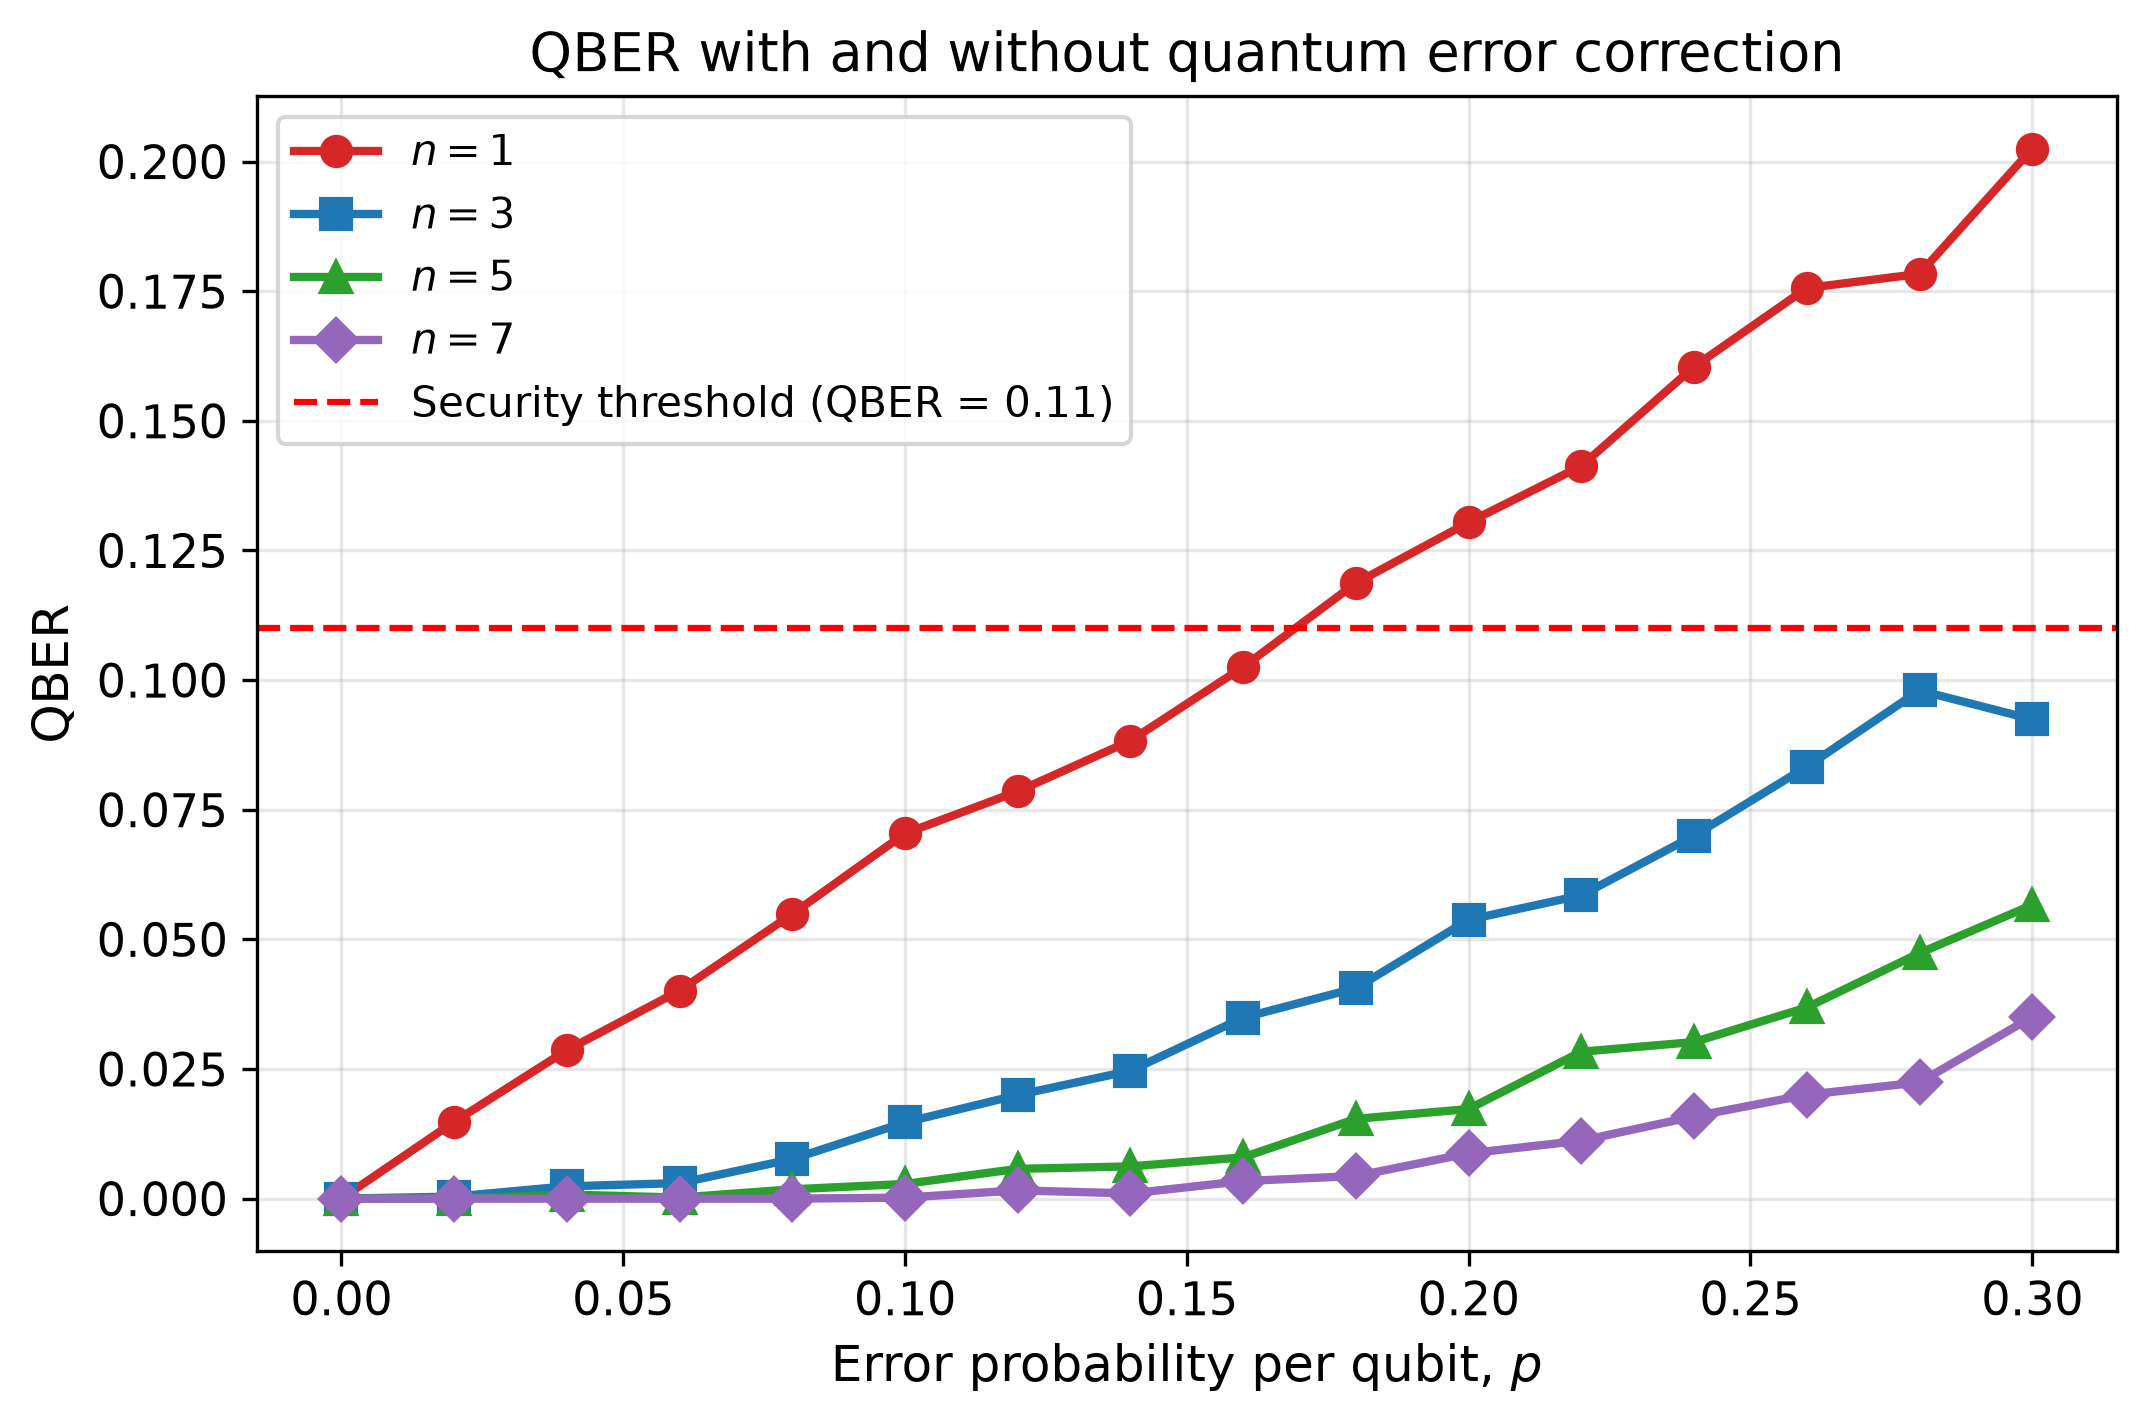
\includegraphics[width=0.85\textwidth]{../figs/qber_vs_p.png}
\caption{QBER en función de la probabilidad de error por qubit \(p\), para
\(n=1\) (sin QEC), \(3\), \(5\) y \(7\). La línea punteada señala el umbral de
seguridad de BB84 (\(\mathrm{QBER}=0.11\)); por encima de él la tasa de clave
secreta es nula. Datos: \texttt{data/resultados\_finales.csv}.}
\label{fig:qber}
\end{figure}

Sin corrección, el QBER crece de forma casi lineal con \(p\), tal como predice la
Ecuación~\eqref{eq:qber}: cada punto de la línea roja se sitúa sobre
\(\mathrm{QBER}=2p/3\). Esa trayectoria corta el umbral en torno a \(p=0.16\), de
manera que a partir de ese nivel de ruido el enlace queda inutilizable por más
que su hardware funcione correctamente. Las tres líneas restantes muestran un
comportamiento muy distinto: se mantienen casi planas y muy por debajo del
umbral. En \(p=0.06\), el QBER desciende de \(0.040\) sin corrección a \(0.003\)
con \(n=3\), es decir, más de diez veces menor; en \(p=0.30\), el escenario más
adverso del barrido, el valor sin corrección es \(0.202\), mientras que con
\(n=3\) es \(0.092\), con \(n=5\) es \(0.057\) y con \(n=7\) es \(0.035\).

La interpretación es directa: la corrección de errores no evita que el canal
dañe los qubits, sino que impide que ese daño se convierta en un error lógico.
El mecanismo es el de la votación descrito en la Sección~1.2.3: al enviar el
mismo valor varias veces y decidir por mayoría, un error aislado no cambia el
resultado, y se requiere que fallen más de la mitad de las copias para que el
dato se pierda. Por eso las curvas de color crecen lentamente y la comunicación
sobrevive a niveles de ruido en los que la operación sin corrección ya se habría
interrumpido. Las pequeñas oscilaciones observadas al final del barrido
(\(p=0.28\) y \(p=0.30\) con \(n=3\)) son compatibles con la variabilidad
estadística del muestreo y no alteran la tendencia.

\subsection{El compromiso (\textit{trade-off}) y el \textit{overhead}}

La Figura~\ref{fig:tasa} muestra la contraparte del resultado anterior. Si la
corrección redujera el QBER sin costo alguno, bastaría con aplicar el código más
grande disponible; la figura demuestra que no es así. La línea roja cae
abruptamente desde la unidad y se anula a partir de \(p=0.18\), mientras que las
líneas de color arrancan mucho más abajo y descienden con suavidad: con
\(n=3\), la tasa se mantiene por encima de \(0.17\) hasta \(p=0.18\) y luego
cae a \(0.037\) en \(p=0.30\); con
\(n=5\), de \(0.200\) a \(0.074\); y con \(n=7\), de \(0.143\) a \(0.080\). Las
curvas se cruzan entre sí, lo que confirma que ningún tamaño de código es
superior en todos los regímenes.

\begin{figure}[H]
\centering
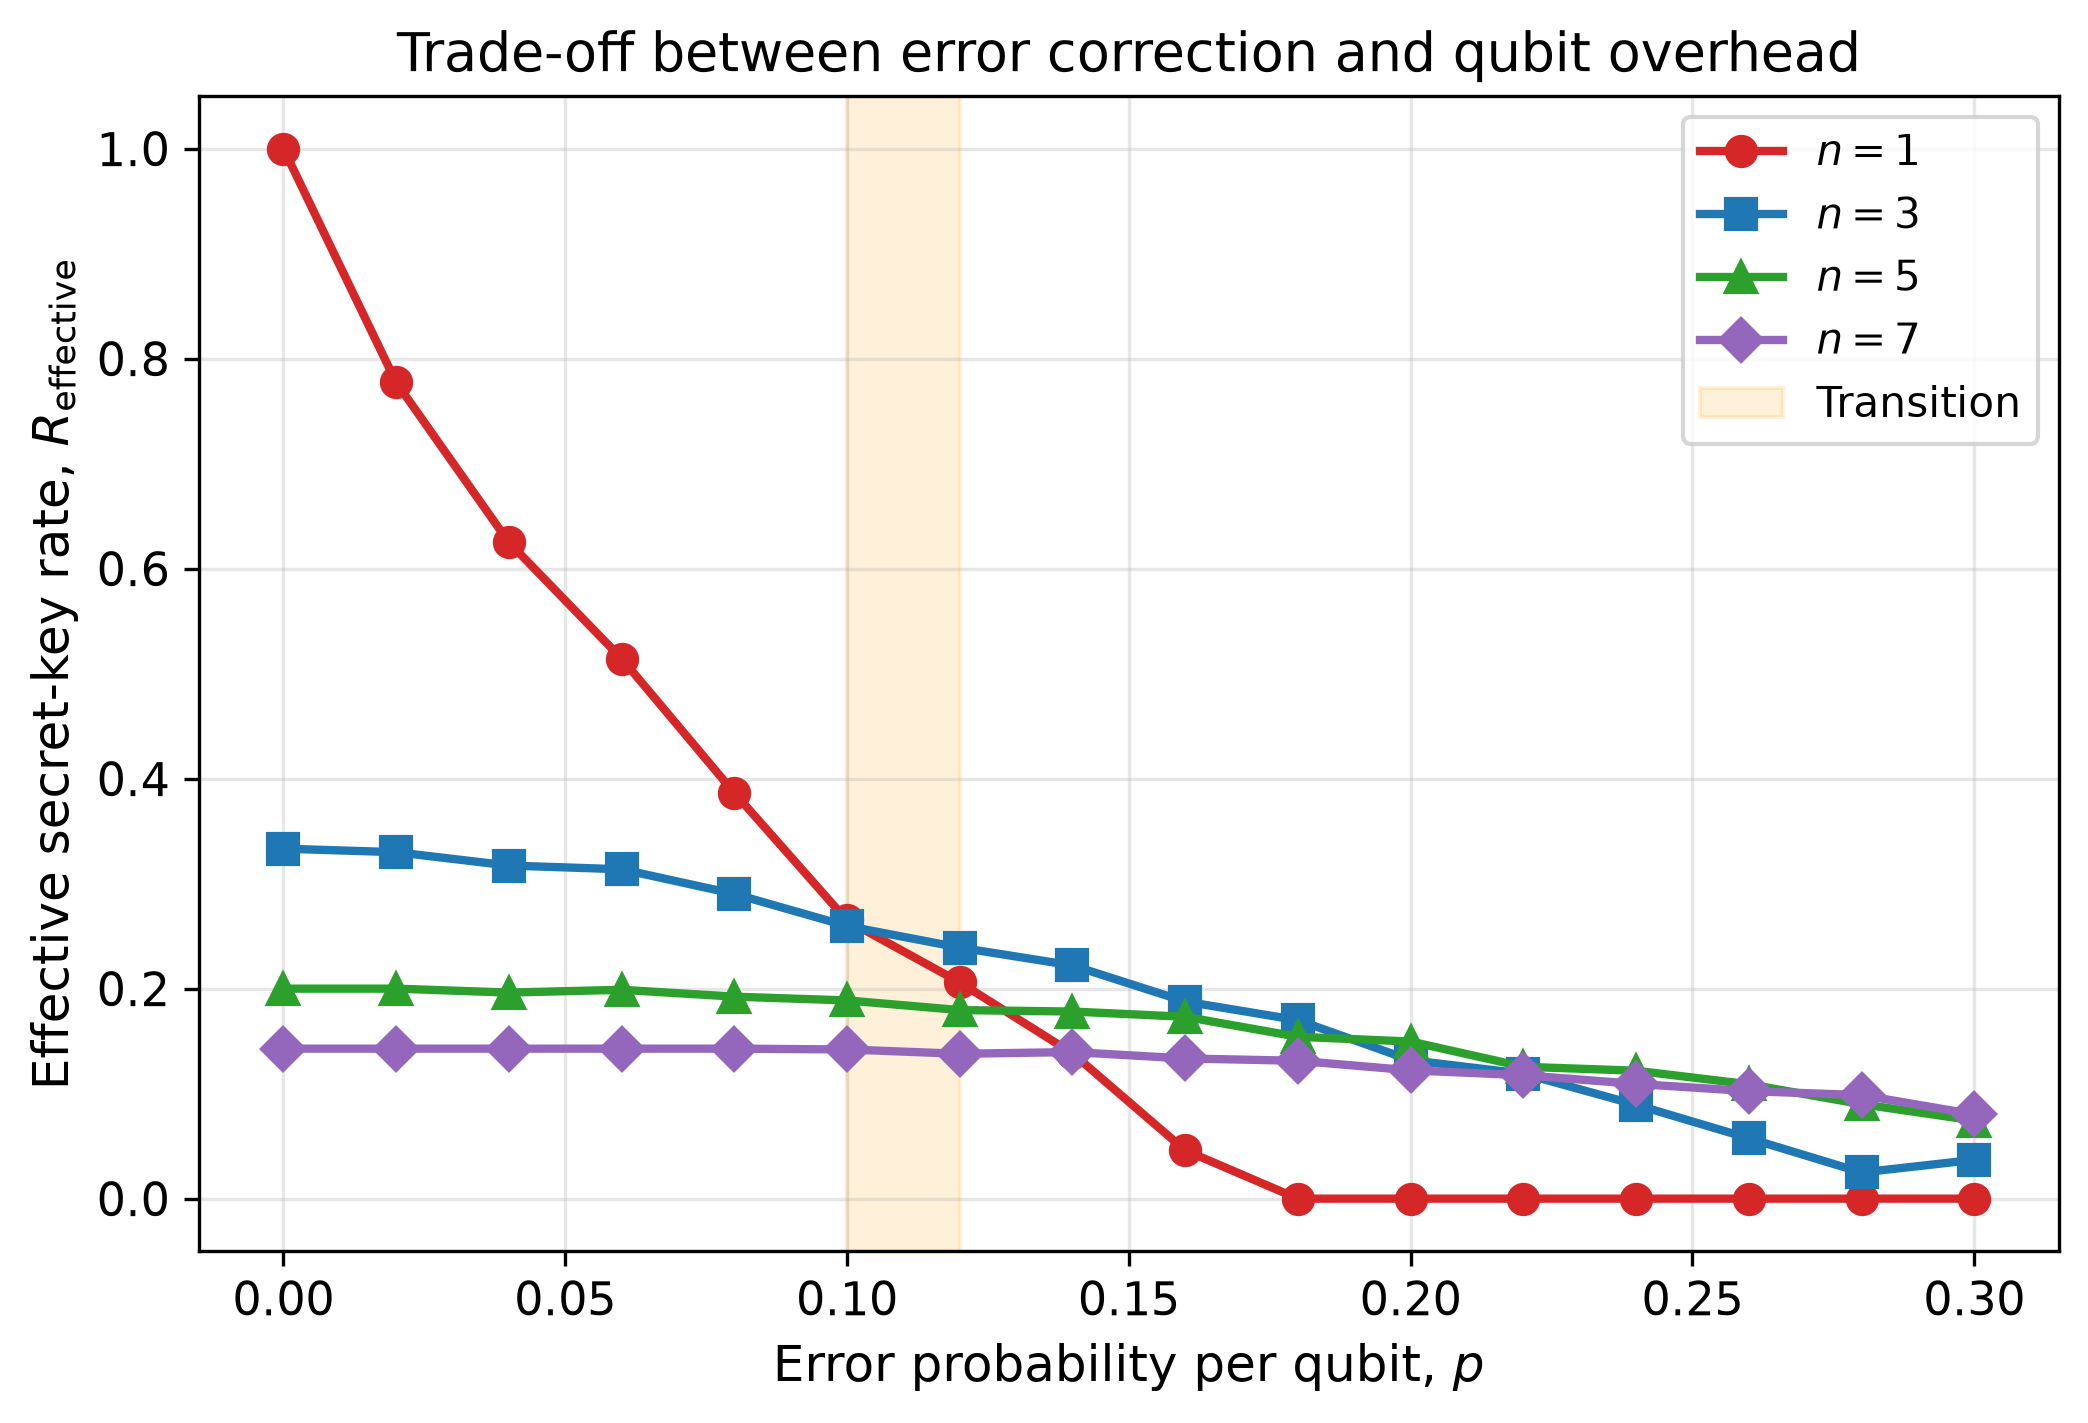
\includegraphics[width=0.85\textwidth]{../figs/tasa_efectiva_vs_p.png}
\caption{Tasa de clave efectiva \(R_{\text{efectiva}}\) en función de \(p\) para
\(n=1,3,5,7\), calculada con la Ecuación~\eqref{eq:efectiva}. La banda naranja
señala la región de transición entre la operación sin corrección y el código
\(n=3\). Datos: \texttt{data/resultados\_finales.csv}.}
\label{fig:tasa}
\end{figure}

El comportamiento se explica con la analogía de los guardias de seguridad
introducida en la Sección~1.2.4. En un barrio tranquilo —un canal con poco
ruido— un solo guardia basta y contratar más solo encarece la operación; en un
barrio peligroso —un canal ruidoso— un guardia resulta insuficiente y el edificio
queda expuesto. La Figura~\ref{fig:tasa} es exactamente esa disyuntiva: a la
izquierda del gráfico manda el ahorro (gana \(n=1\), porque el QBER aún es bajo y
no hace falta proteger nada), y a la derecha manda la protección (ganan \(n=3\),
\(5\) y \(7\), porque sin guardias no queda clave que repartir). Cada guardia
adicional consume recursos que dejan de destinarse a transmitir información, y de
ahí que las curvas de los códigos grandes nunca alcancen a la del código pequeño
en la zona de bajo ruido.

La Tabla~\ref{tab:optimo} resume la decisión óptima para cada nivel de ruido,
obtenida al seleccionar, para cada \(p\), el tamaño de código que maximiza la
Ecuación~\eqref{eq:efectiva}. Los valores provienen de
\texttt{data/n\_optimo.csv}.

\begin{table}[H]
\centering
\caption{Tamaño de código óptimo \(n^{*}\) y tasa de clave efectiva alcanzada
\(R_{\text{efectiva}}(p,n^{*})\), para cada nivel de ruido \(p\).}
\label{tab:optimo}
\small
\begin{tabular}{@{}cccc@{}}
\toprule
\(p\) & \(n^{*}\) & \(R_{\text{efectiva}}(p,n^{*})\) & Régimen \\
\midrule
0.00 & 1 & 1.0000 & \multirow{6}{*}{Sin QEC} \\
0.02 & 1 & 0.7775 & \\
0.04 & 1 & 0.6251 & \\
0.06 & 1 & 0.5144 & \\
0.08 & 1 & 0.3865 & \\
0.10 & 1 & 0.2650 & \\
\midrule
0.12 & 3 & 0.2391 & \multirow{4}{*}{Código \(n=3\)} \\
0.14 & 3 & 0.2221 & \\
0.16 & 3 & 0.1877 & \\
0.18 & 3 & 0.1700 & \\
\midrule
0.20 & 5 & 0.1496 & \multirow{4}{*}{Código \(n=5\)} \\
0.22 & 5 & 0.1256 & \\
0.24 & 5 & 0.1218 & \\
0.26 & 5 & 0.1089 & \\
\midrule
0.28 & 7 & 0.0986 & \multirow{2}{*}{Código \(n=7\)} \\
0.30 & 7 & 0.0802 & \\
\bottomrule
\end{tabular}
\end{table}

La lectura de la tabla delimita cuatro regímenes. Hasta \(p=0.10\) conviene no
aplicar corrección: el QBER permanece por debajo del umbral y cualquier código
reduce la tasa a un tercio o menos de su valor. Entre \(p=0.12\) y \(p=0.18\) el
óptimo es \(n=3\), que conserva una tasa entre \(0.239\) y \(0.170\) en una zona
donde la operación sin corrección ya se ha degradado severamente o se ha anulado.
Entre \(p=0.20\) y \(p=0.26\) el óptimo pasa a \(n=5\), y a partir de \(p=0.28\) a
\(n=7\). El costo de equivocarse en la elección no es menor: en \(p=0.12\),
aplicar \(n=7\) en lugar de \(n=3\) exigiría más del doble de qubits físicos por
qubit lógico y, aun así, entregaría una tasa de \(0.138\) frente a \(0.239\);
en \(p=0.18\), operar sin corrección entrega una tasa nula, mientras que \(n=3\)
entrega \(0.170\).

\subsection{Mapa de calor \((p,n)\)}

La Figura~\ref{fig:mapa} presenta la misma información en forma de mapa de calor,
lo que permite apreciar de un solo vistazo la estructura del compromiso. Cada
fila corresponde a un tamaño de código y cada columna a un nivel de ruido; el
color de cada celda representa la tasa efectiva, con la escala \textit{viridis}
que va del morado oscuro (valores cercanos a cero) al amarillo (valor máximo de
la escala, \(1.0\)). Las celdas incluyen además el valor numérico, de modo que la
figura puede leerse sin depender del color.

\begin{figure}[H]
\centering
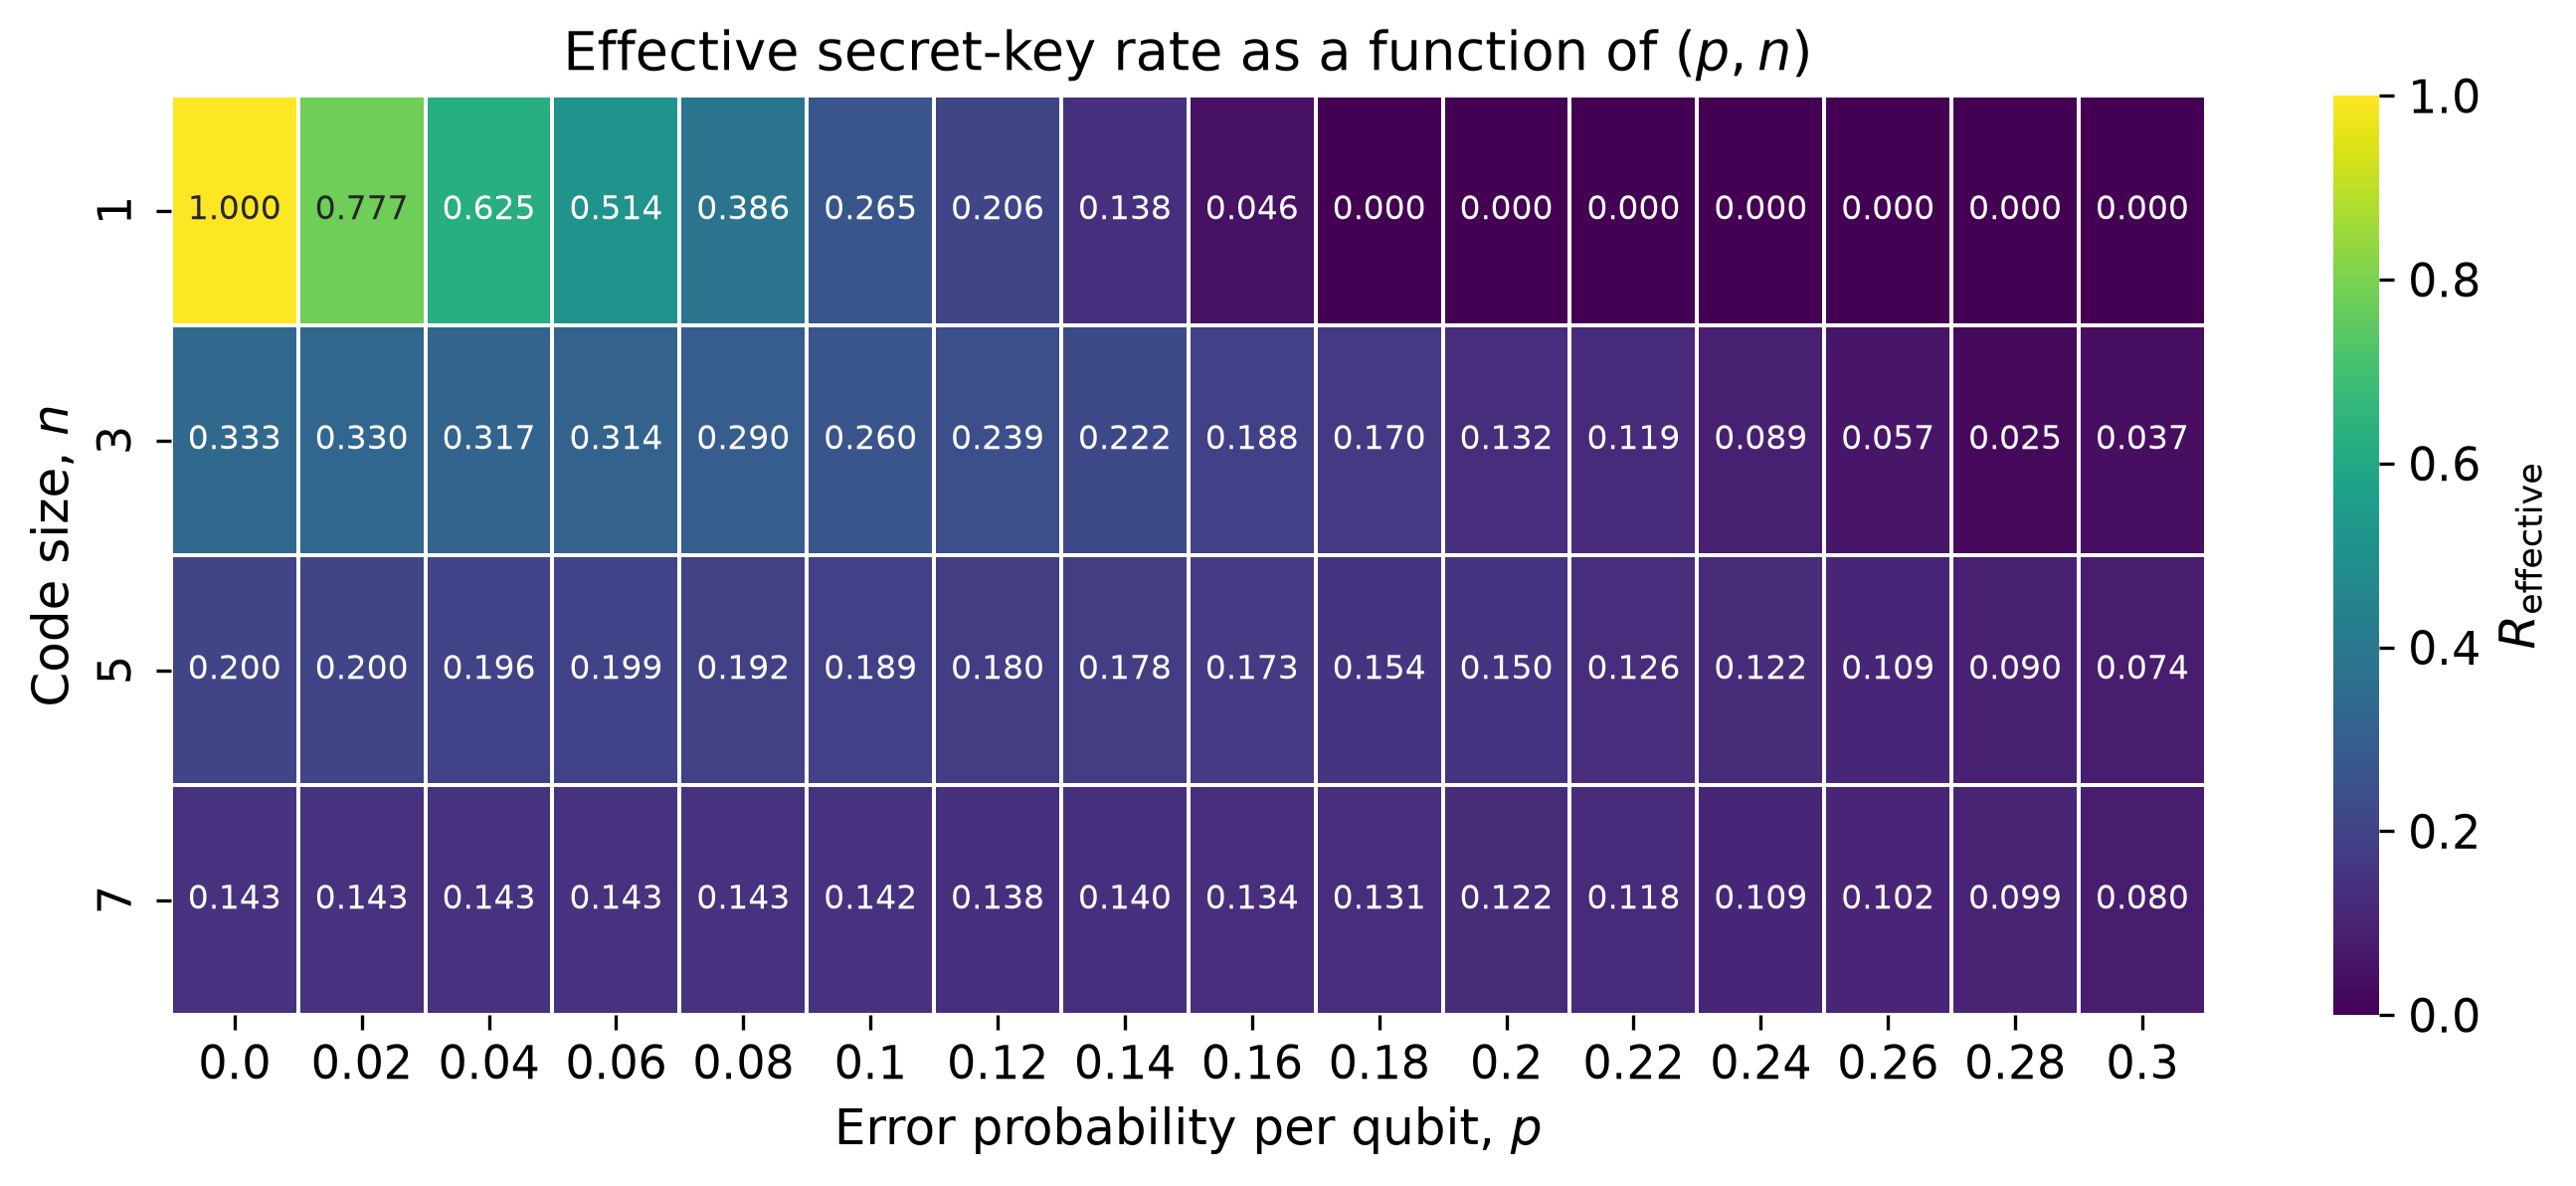
\includegraphics[width=\textwidth]{../figs/mapa_calor.png}
\caption{Tasa de clave efectiva \(R_{\text{efectiva}}\) en función de \((p,n)\);
el color más claro indica mayor tasa. La celda más brillante de cada columna
señala el código óptimo para ese nivel de ruido. Datos:
\texttt{data/resultados\_finales.csv}.}
\label{fig:mapa}
\end{figure}

La transición de colores cuenta la historia del proyecto. En la primera fila
(\(n=1\)) se observa un degradado continuo y rápido: amarillo intenso en \(p=0\),
verde en \(p=0.02\) y \(p=0.04\), turquesa en \(p=0.06\), azul en \(p=0.10\) y
morado uniforme desde \(p=0.16\), donde la tasa se anula. Las filas restantes, en
cambio, son casi monocromáticas: permanecen en tonos azules y morados a lo largo
de todo el eje horizontal, lo que significa que su tasa varía poco con el ruido.
Esa diferencia visual es la esencia de la corrección: sin QEC, el rendimiento
depende críticamente del canal; con QEC, se vuelve estable.

El rasgo más informativo del mapa es el desplazamiento de la celda más clara de
cada columna. Para \(p=0\) el máximo está en la fila \(n=1\); para \(p=0.02\) a
\(p=0.10\) sigue en \(n=1\); a partir de \(p=0.12\) el valor más alto de la
columna se traslada a \(n=3\) (\(0.239\) frente a \(0.206\) de \(n=1\)); en
\(p=0.20\) se traslada a \(n=5\) (\(0.150\) frente a \(0.132\) de \(n=3\)); y en
\(p=0.28\) a \(n=7\) (\(0.099\) frente a \(0.090\) de \(n=5\)). Ese descenso
escalonado dibuja una diagonal que responde la pregunta de investigación: el
tamaño de código óptimo aumenta con el ruido, y lo hace por escalones, no de
forma continua, porque solo se dispone de cuatro tamaños en el conjunto evaluado.

\section{Discusión}

Los resultados obtenidos dialogan de forma directa con los antecedentes
revisados. \citet{jha2024} propusieron integrar el cifrado y la corrección de
errores mediante códigos CSS con el propósito de reducir el costo total al reunir
ambas funciones en un mismo proceso. Los datos de este proyecto confirman la
premisa de ese planteamiento —el \textit{overhead} es la restricción dominante,
no la capacidad de corrección— y permiten cuantificarla con precisión: el factor
\(1/n\) de la Ecuación~\eqref{eq:efectiva} impone que duplicar la protección
reduzca a la mitad el rendimiento, de modo que el costo no se elimina, sino que
se administra eligiendo el bloque adecuado. La contribución de Jha y
colaboradores opera sobre el costo fijo del sistema (las etapas separadas de
cifrado y corrección); la de este trabajo opera sobre el costo variable (el
tamaño del bloque en función del ruido). Son enfoques complementarios: un sistema
que integre ambas funciones seguiría necesitando el criterio \(n^{*}(p)\) para
dimensionarse, y viceversa. La diferencia de alcance explica también por qué
nuestros resultados no contradicen los suyos aunque partan de supuestos distintos:
ellos evalúan la viabilidad de una arquitectura integrada, mientras que aquí se
evalúa la frontera de optimalidad en un protocolo concreto.

La comparación con el trabajo del equipo de Google Quantum AI
\citep{google2025} exige una precisión adicional, porque opera en un régimen
distinto. Aquellos autores demostraron la supresión del error lógico por debajo
del umbral del código de superficie en un procesador superconductor de 105
qubits, con lo que validaron experimentalmente la viabilidad de la corrección de
errores a gran escala. Ese resultado respalda la dirección general de esta
investigación, pero no es directamente trasladable: allí el objetivo es la
fidelidad de un computador tolerante a fallos, con decenas o centenares de qubits
físicos por qubit lógico, mientras que aquí se protege un enlace de QKD en el que
solo se necesita preservar el bit transmitido y donde un código de tres qubits ya
produce ganancias medibles. Lo que sí se transfiere es la noción de umbral: por
debajo de cierto nivel de ruido, proteger más no compensa —y eso es exactamente
lo que muestra el predominio de \(n=1\) hasta \(p=0.10\)—, mientras que por encima
la protección se vuelve imprescindible. La diferencia radica en la métrica: ellos
optimizan fidelidad, este trabajo optimiza tasa de clave efectiva con un costo
explícito en qubits.

Desde la perspectiva de la ciberseguridad, los resultados tienen dos
consecuencias prácticas. La primera es la extensión del rango operativo. Sin
corrección, el enlace deja de generar clave cuando la probabilidad de error
alcanza \(p \approx 0.165\) (Ecuación~\eqref{eq:qber} en la
Ecuación~\eqref{eq:shor}); con \(n=3\), el umbral no se alcanza ni siquiera en
\(p=0.30\), el extremo del barrido. Dicho de otro modo, la corrección
aproximadamente duplica la tolerancia al ruido del canal y, como la probabilidad
de error crece en primera aproximación con la distancia recorrida en la fibra,
ese margen se traduce en un alcance útil cercano al doble del que tendría el
mismo enlace sin protección. La segunda es el ahorro de hardware. Aplicar
sistemáticamente el código más protector disponible —la decisión intuitiva—
derrocha recursos: en \(p=0.12\), usar \(n=7\) exige más del doble de qubits
físicos por qubit lógico y entrega \(0.138\) en lugar de los \(0.239\) que
alcanza \(n=3\) con tres qubits. Elegir \(n^{*}(p)\) permite obtener más clave con
menos hardware, o dicho en términos de seguridad, evita prometer una capacidad de
generación que el enlace no puede sostener. Esta última consideración es
especialmente relevante en un contexto de migración criptográfica, donde una
sobreestimación de la tasa de clave se traduce en garantías de confidencialidad
que el sistema no puede cumplir. Conviene subrayar, no obstante, que estas
conclusiones corresponden a un modelo idealizado —canal depolarizante, fuentes y
detectores perfectos y régimen asintótico— y que su traslado a enlaces reales
requiere la validación experimental que se señala en el apartado de limitaciones.

\section{Conclusiones}
El presente proyecto demostró que no existe un tamaño de código QEC universal, sino que depende del ruido del canal. Se identificó que para \(p \le 0.10\) no se requiere QEC, mientras que para \(0.12 \le p \le 0.18\) el código \(n=3\) es óptimo, para \(0.20 \le p \le 0.26\) lo es \(n=5\) y a partir de \(p \ge 0.28\) domina \(n=7\).

\section{Limitaciones y recomendaciones}
\begin{itemize}
    \item El código de repetición implementado solo corrige errores de bit-flip (X), no errores de fase (Z).
    \item Trabajo futuro: Evaluar códigos estabilizadores más complejos (Steane, Superficie).
\end{itemize}

% ------------------------------------------------------------
% ANEXOS Y REFERENCIAS
% ------------------------------------------------------------
\appendix
\chapter{Anexos}

\section{Declaración de uso de IA}
La presente investigación ha sido apoyada por herramientas de inteligencia artificial (DeepSeek, modelos locales Qwen y Gemma) para la organización de ideas, redacción y validación de referencias. Se mantuvo en todo momento un monitoreo y comprobación de las fuentes, el código y los resultados.

\section{Repositorio de evidencias}
El código fuente, los datos crudos (CSV) y las figuras pueden ser consultados en el repositorio de GitHub: \\
\url{https://github.com/em-path/quantum-qec-bb84-analysis}

\section{Código fuente principal}

Esta sección reproduce los dos módulos centrales del paquete de reproducción
(\texttt{reproduction\_package/}), una versión autocontenida del código, con
documentación en inglés y sin dependencias del entorno de desarrollo original.
El Listado~\ref{lst:qec} presenta el módulo de corrección de errores
---codificación, medición de síndromes, corrección y decodificación--- y el
Listado~\ref{lst:simulacion} el flujo integrado, que ejecuta el protocolo BB84,
aplica el canal depolarizante, calcula el QBER y obtiene la tasa de clave
efectiva. Ambos archivos se ejecutan con Python 3.14 y QuTiP 5.0.

\newpage

\lstinputlisting[style=pythonstyle,
    caption={Módulo de corrección de errores cuánticos (\texttt{qec.py}):
    codificación, medición de síndromes, corrección y decodificación del código
    de repetición.},
    label={lst:qec}]
    {../src/qec.py}

\newpage

\lstinputlisting[style=pythonstyle,
    caption={Simulación integrada (\texttt{simulation.py}): protocolo BB84,
    canal depolarizante y cálculo de la tasa de clave efectiva.},
    label={lst:simulacion}]
    {../src/simulation.py}

% ------------------------------------------------------------
% ANEXO B: ARTÍCULO ACADÉMICO
% ------------------------------------------------------------
\chapter{Artículo académico}
\label{anexo:articulo}

El artículo que se reproduce a continuación sintetiza los resultados de este
proyecto en el formato de una comunicación académica de cinco páginas,
estructurada conforme al estilo IEEE para congresos. Se incorpora como anexo en
cumplimiento de la guía de entrega, que exige adjuntar el artículo derivado del
PIA, y constituye una versión autosuficiente del problema, el método, los
resultados y las conclusiones ya expuestos en los capítulos precedentes.

\begin{itemize}
    \item \textbf{Título:} «Corrección de errores cuánticos y tasa de clave
    segura en BB84 bajo canales ruidosos».
    \item \textbf{Formato:} comunicación de congreso elaborada con la clase
    \texttt{IEEEtran} (opción \texttt{conference}); cinco páginas.
    \item \textbf{Estructura:} resumen y palabras clave, introducción,
    antecedentes, método, resultados y conclusiones, con tres figuras y dos
    tablas.
    \item \textbf{Relación con el PIA:} reproduce el problema, el método y los
    resultados de los Capítulos~I a~III, con su propia lista de referencias en
    estilo IEEE.
    \item \textbf{Disponibilidad:} el archivo fuente
    (\texttt{articulo\_ieee.tex}) y su versión compilada
    (\texttt{articulo\_ieee.pdf}) se conservan en el repositorio de evidencias
    descrito en el Anexo~A.
\end{itemize}

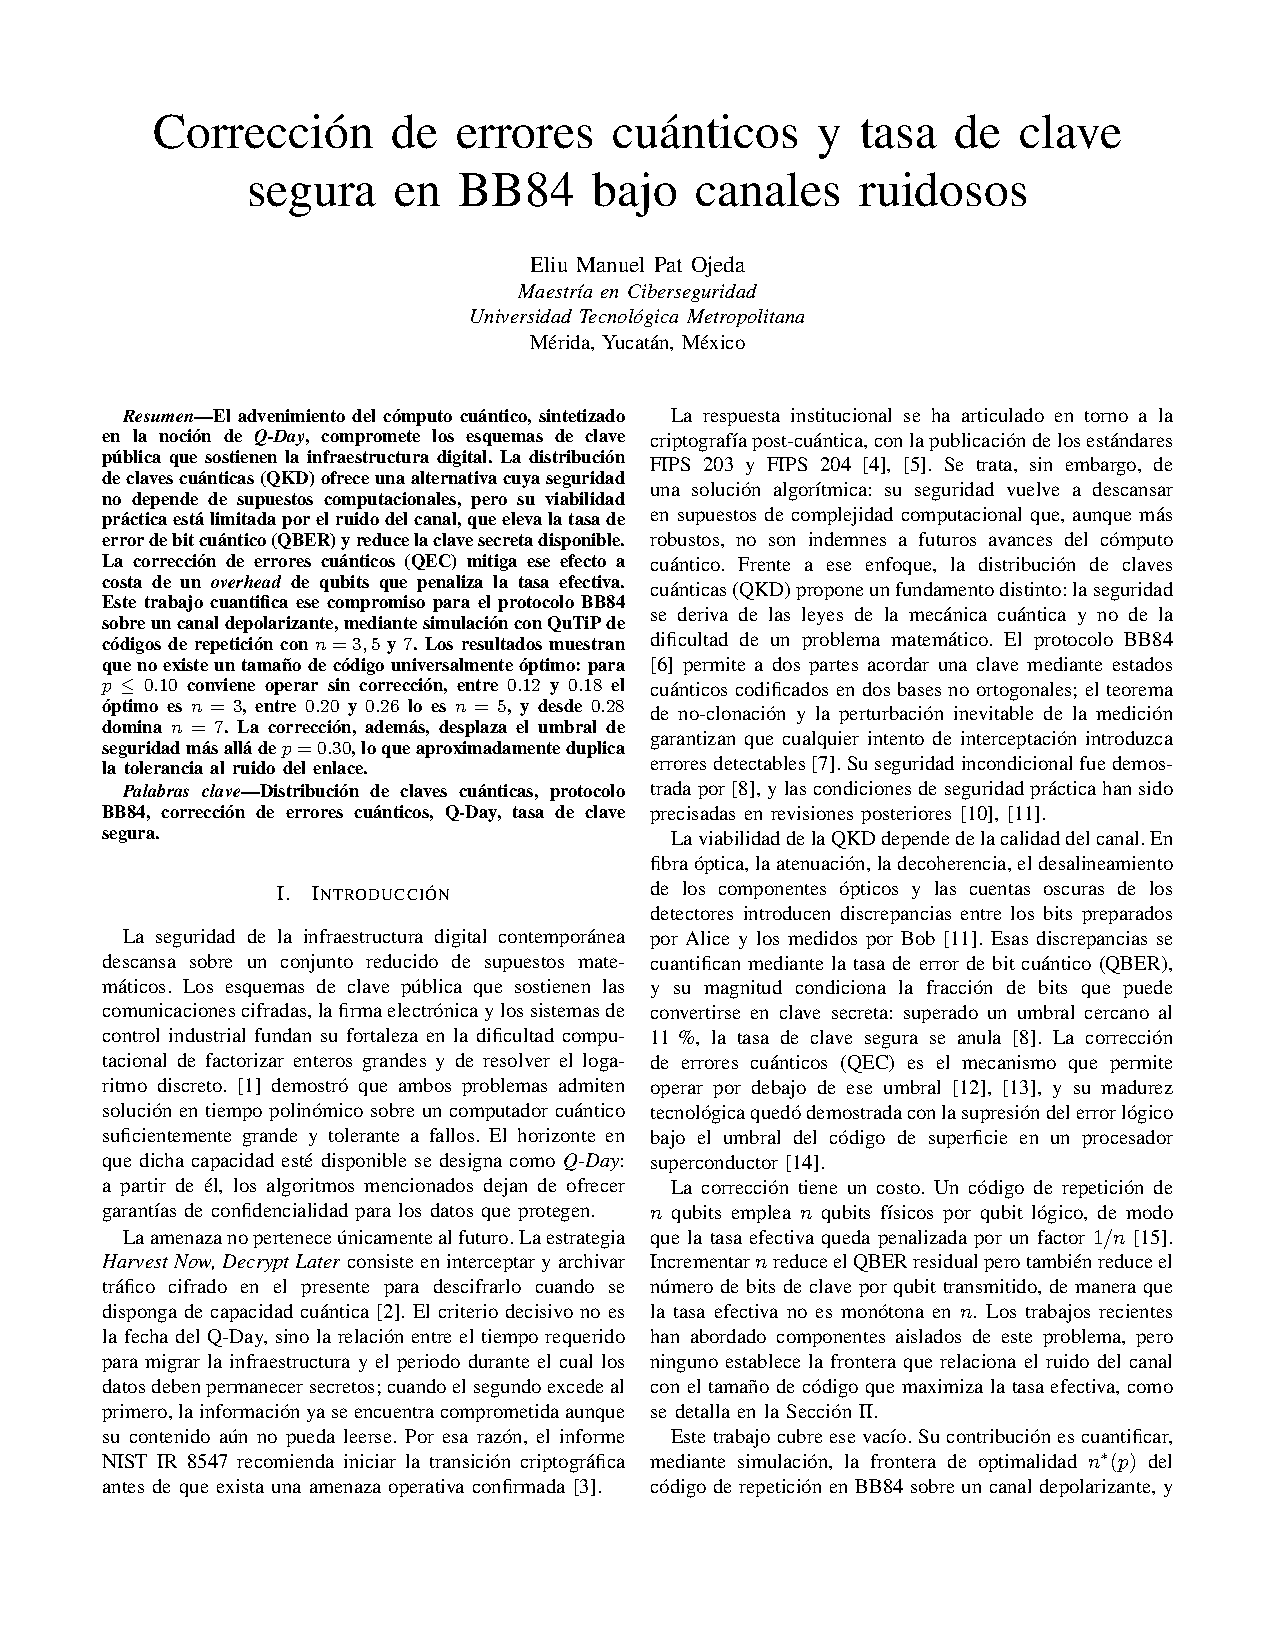
\includepdf[pages=-, landscape=false]{articulo_ieee.pdf}

% ============================================================
% REFERENCIAS (APA 7)
% ============================================================
\renewcommand{\bibname}{Referencias}
\phantomsection
\addcontentsline{toc}{chapter}{Referencias}
\begin{thebibliography}{99}

\bibitem[Acharya et al.(2025)]{google2025} Acharya, R., et al. [Google Quantum AI and Collaborators]. (2025). Quantum error correction below the surface code threshold. \textit{Nature}, \textit{638}(8052), 920-926. \url{https://doi.org/10.1038/s41586-024-08449-y}

\bibitem[Bennett y Brassard(1984)]{bennett1984} Bennett, C. H., \& Brassard, G. (1984). Quantum cryptography: Public key distribution and coin tossing. En \textit{Proceedings of the IEEE International Conference on Computers, Systems and Signal Processing} (pp. 175-179). IEEE. Reimpresión en \textit{Theoretical Computer Science}, \textit{560}, 7-11 (2014). \url{https://doi.org/10.1016/j.tcs.2014.05.025}

\bibitem[Calderbank y Shor(1996)]{calderbank1996} Calderbank, A. R., \& Shor, P. W. (1996). Good quantum error-correcting codes exist. \textit{Physical Review A}, \textit{54}(2), 1098-1105. \url{https://doi.org/10.1103/PhysRevA.54.1098}

\bibitem[Devetak y Winter(2005)]{devetak2005} Devetak, I., \& Winter, A. (2005). Distillation of secret key and entanglement from quantum states. \textit{Proceedings of the Royal Society A}, \textit{461}(2053), 207-235. \url{https://doi.org/10.1098/rspa.2004.1372}

\bibitem[Fowler et al.(2012)]{fowler2012} Fowler, A. G., Mariantoni, M., Martinis, J. M., \& Cleland, A. N. (2012). Surface codes: Towards practical large-scale quantum computation. \textit{Physical Review A}, \textit{86}(3), 032324. \url{https://doi.org/10.1103/PhysRevA.86.032324}

\bibitem[Gisin et al.(2002)]{gisin2002} Gisin, N., Ribordy, G., Tittel, W., \& Zbinden, H. (2002). Quantum cryptography. \textit{Reviews of Modern Physics}, \textit{74}(1), 145-195. \url{https://doi.org/10.1103/RevModPhys.74.145}

\bibitem[Gottesman(1997)]{gottesman1997} Gottesman, D. (1997). Stabilizer codes and quantum error correction. \textit{arXiv preprint quant-ph/9705052}. \url{https://doi.org/10.48550/arXiv.quant-ph/9705052}

\bibitem[Jayachandran y Malathi(2025)]{jayachandran2025} Jayachandran, R., \& Malathi, D. (2025). Experimental validation of quantum error correction in BB84 for secure quantum communication. \textit{International Journal of Theoretical Physics}, \textit{64}(11), 310. \url{https://doi.org/10.1007/s10773-025-06148-6}

\bibitem[Jha et al.(2024)]{jha2024} Jha, N., Parakh, A., \& Subramaniam, M. (2024). Joint encryption and error correction for secure quantum communication. \textit{Scientific Reports}, \textit{14}, 24542. \url{https://doi.org/10.1038/s41598-024-75212-8}

\bibitem[Johansson et al.(2012)]{qutip2012} Johansson, J. R., Nation, P. D., \& Nori, F. (2012). QuTiP: An open-source Python framework for the dynamics of open quantum systems. \textit{Computer Physics Communications}, \textit{183}(8), 1760-1772. \url{https://doi.org/10.1016/j.cpc.2012.02.021}

\bibitem[Lo et al.(2014)]{lo2014} Lo, H.-K., Curty, M., \& Tamaki, K. (2014). Secure quantum key distribution. \textit{Nature Photonics}, \textit{8}(8), 595-604. \url{https://doi.org/10.1038/nphoton.2014.149}

\bibitem[Matsui y Kaneko(2025)]{matsui2025} Matsui, H., \& Kaneko, K. (2025). Entanglement-assisted quantum error-correcting codes via quasi-cyclic codes with complementary duals. \textit{Designs, Codes and Cryptography}, \textit{93}(9), 3575-3591. \url{https://doi.org/10.1007/s10623-025-01650-8}

\bibitem[Mosca(2018)]{mosca2018} Mosca, M. (2018). Cybersecurity in an era with quantum computers: Will we be ready? \textit{IEEE Security \& Privacy}, \textit{16}(5), 38-41. \url{https://doi.org/10.1109/MSP.2018.3761723}

\bibitem[Nielsen y Chuang(2010)]{nielsen2010} Nielsen, M. A., \& Chuang, I. L. (2010). \textit{Quantum computation and quantum information} (10.\textsuperscript{a} ed. conmemorativa). Cambridge University Press. \url{https://doi.org/10.1017/CBO9780511976667}

\bibitem[NIST(2024a)]{nist2024a} National Institute of Standards and Technology. (2024a). \textit{Module-lattice-based key-encapsulation mechanism standard} (FIPS 203). U.S. Department of Commerce. \url{https://doi.org/10.6028/NIST.FIPS.203}

\bibitem[NIST(2024b)]{nist2024b} National Institute of Standards and Technology. (2024b). \textit{Module-lattice-based digital signature standard} (FIPS 204). U.S. Department of Commerce. \url{https://doi.org/10.6028/NIST.FIPS.204}

\bibitem[Regenscheid(2026)]{nist2026ir} Regenscheid, A. (2026). \textit{Transition to post-quantum cryptography standards} (NIST IR 8547). National Institute of Standards and Technology. \url{https://doi.org/10.6028/NIST.IR.8547}

\bibitem[Pirandola et al.(2020)]{pirandola2020} Pirandola, S., Andersen, U. L., Banchi, L., Berta, M., Bunandar, D., Colbeck, R., Englund, D., Gehring, T., Lupo, C., Ottaviani, C., Pereira, J. L., Razavi, M., Shamsul Shaari, J., Tomamichel, M., Usenko, V. C., Vallone, G., Villoresi, P., \& Wallden, P. (2020). Advances in quantum cryptography. \textit{Advances in Optics and Photonics}, \textit{12}(4), 1012-1236. \url{https://doi.org/10.1364/AOP.361502}

\bibitem[Preskill(2018)]{preskill2018} Preskill, J. (2018). Quantum computing in the NISQ era and beyond. \textit{Quantum}, \textit{2}, 79. \url{https://doi.org/10.22331/q-2018-08-06-79}

\bibitem[Roffe(2019)]{roffe2019} Roffe, J. (2019). Quantum error correction: An introductory guide. \textit{Contemporary Physics}, \textit{60}(3), 226-245. \url{https://doi.org/10.1080/00107514.2019.1667078}

\bibitem[Scarani et al.(2009)]{scarani2009} Scarani, V., Bechmann-Pasquinucci, H., Cerf, N. J., Du\v{s}ek, M., L\"utkenhaus, N., \& Peev, M. (2009). The security of practical quantum key distribution. \textit{Reviews of Modern Physics}, \textit{81}(3), 1301-1350. \url{https://doi.org/10.1103/RevModPhys.81.1301}

\bibitem[Shor(1997)]{shor1997} Shor, P. W. (1997). Polynomial-time algorithms for prime factorization and discrete logarithms on a quantum computer. \textit{SIAM Journal on Computing}, \textit{26}(5), 1484-1509. \url{https://doi.org/10.1137/S0097539795293172}

\bibitem[Shor y Preskill(2000)]{shor2000} Shor, P. W., \& Preskill, J. (2000). Simple proof of security of the BB84 quantum key distribution protocol. \textit{Physical Review Letters}, \textit{85}(2), 441-444. \url{https://doi.org/10.1103/PhysRevLett.85.441}

\bibitem[Steane(1996)]{steane1996} Steane, A. M. (1996). Error correcting codes in quantum theory. \textit{Physical Review Letters}, \textit{77}(5), 793-797. \url{https://doi.org/10.1103/PhysRevLett.77.793}

\bibitem[Terhal(2015)]{terhal2015} Terhal, B. M. (2015). Quantum error correction for quantum memories. \textit{Reviews of Modern Physics}, \textit{87}(2), 307-346. \url{https://doi.org/10.1103/RevModPhys.87.307}

\bibitem[Xu et al.(2020)]{xu2020} Xu, F., Ma, X., Zhang, Q., Lo, H.-K., \& Pan, J.-W. (2020). Secure quantum key distribution with realistic devices. \textit{Reviews of Modern Physics}, \textit{92}(2), 025002. \url{https://doi.org/10.1103/RevModPhys.92.025002}

\bibitem[Zheng et al.(2024)]{zheng2024} Zheng, G., He, W., Lee, G., \& Jiang, L. (2024). Near-optimal performance of quantum error correction codes. \textit{Physical Review Letters}, \textit{132}(25), 250602. \url{https://doi.org/10.1103/PhysRevLett.132.250602}

\end{thebibliography}

\end{document}